\documentclass[twoside]{book}

% Packages required by doxygen
\usepackage{fixltx2e}
\usepackage{calc}
\usepackage{doxygen}
\usepackage[export]{adjustbox} % also loads graphicx
\usepackage{graphicx}
\usepackage[utf8]{inputenc}
\usepackage{makeidx}
\usepackage{multicol}
\usepackage{multirow}
\PassOptionsToPackage{warn}{textcomp}
\usepackage{textcomp}
\usepackage[nointegrals]{wasysym}
\usepackage[table]{xcolor}

% Font selection
\usepackage[T1]{fontenc}
\usepackage[scaled=.90]{helvet}
\usepackage{courier}
\usepackage{amssymb}
\usepackage{sectsty}
\renewcommand{\familydefault}{\sfdefault}
\allsectionsfont{%
  \fontseries{bc}\selectfont%
  \color{darkgray}%
}
\renewcommand{\DoxyLabelFont}{%
  \fontseries{bc}\selectfont%
  \color{darkgray}%
}
\newcommand{\+}{\discretionary{\mbox{\scriptsize$\hookleftarrow$}}{}{}}

% Page & text layout
\usepackage{geometry}
\geometry{%
  a4paper,%
  top=2.5cm,%
  bottom=2.5cm,%
  left=2.5cm,%
  right=2.5cm%
}
\tolerance=750
\hfuzz=15pt
\hbadness=750
\setlength{\emergencystretch}{15pt}
\setlength{\parindent}{0cm}
\setlength{\parskip}{3ex plus 2ex minus 2ex}
\makeatletter
\renewcommand{\paragraph}{%
  \@startsection{paragraph}{4}{0ex}{-1.0ex}{1.0ex}{%
    \normalfont\normalsize\bfseries\SS@parafont%
  }%
}
\renewcommand{\subparagraph}{%
  \@startsection{subparagraph}{5}{0ex}{-1.0ex}{1.0ex}{%
    \normalfont\normalsize\bfseries\SS@subparafont%
  }%
}
\makeatother

% Headers & footers
\usepackage{fancyhdr}
\pagestyle{fancyplain}
\fancyhead[LE]{\fancyplain{}{\bfseries\thepage}}
\fancyhead[CE]{\fancyplain{}{}}
\fancyhead[RE]{\fancyplain{}{\bfseries\leftmark}}
\fancyhead[LO]{\fancyplain{}{\bfseries\rightmark}}
\fancyhead[CO]{\fancyplain{}{}}
\fancyhead[RO]{\fancyplain{}{\bfseries\thepage}}
\fancyfoot[LE]{\fancyplain{}{}}
\fancyfoot[CE]{\fancyplain{}{}}
\fancyfoot[RE]{\fancyplain{}{\bfseries\scriptsize Generated by Doxygen }}
\fancyfoot[LO]{\fancyplain{}{\bfseries\scriptsize Generated by Doxygen }}
\fancyfoot[CO]{\fancyplain{}{}}
\fancyfoot[RO]{\fancyplain{}{}}
\renewcommand{\footrulewidth}{0.4pt}
\renewcommand{\chaptermark}[1]{%
  \markboth{#1}{}%
}
\renewcommand{\sectionmark}[1]{%
  \markright{\thesection\ #1}%
}

% Indices & bibliography
\usepackage{natbib}
\usepackage[titles]{tocloft}
\setcounter{tocdepth}{3}
\setcounter{secnumdepth}{5}
\makeindex

% Hyperlinks (required, but should be loaded last)
\usepackage{ifpdf}
\ifpdf
  \usepackage[pdftex,pagebackref=true]{hyperref}
\else
  \usepackage[ps2pdf,pagebackref=true]{hyperref}
\fi
\hypersetup{%
  colorlinks=true,%
  linkcolor=blue,%
  citecolor=blue,%
  unicode%
}

% Custom commands
\newcommand{\clearemptydoublepage}{%
  \newpage{\pagestyle{empty}\cleardoublepage}%
}

\usepackage{caption}
\captionsetup{labelsep=space,justification=centering,font={bf},singlelinecheck=off,skip=4pt,position=top}

%===== C O N T E N T S =====

\begin{document}

% Titlepage & ToC
\hypersetup{pageanchor=false,
             bookmarksnumbered=true,
             pdfencoding=unicode
            }
\pagenumbering{alph}
\begin{titlepage}
\vspace*{7cm}
\begin{center}%
{\Large M\+G2\+Modeller++ }\\
\vspace*{1cm}
{\large Generated by Doxygen 1.8.13}\\
\end{center}
\end{titlepage}
\clearemptydoublepage
\pagenumbering{roman}
\tableofcontents
\clearemptydoublepage
\pagenumbering{arabic}
\hypersetup{pageanchor=true}

%--- Begin generated contents ---
\chapter{mg2modeller++}
\label{md_README}
\Hypertarget{md_README}
A 3d modeller inspired by Caligari Truespace and another popular 3d modelling tool. Written in G\+TK and C++.



Development Notes\+: Primarily developed using Code\+Lite I\+DE, can be built using either the C\+LI or Code\+Lite. Simply type Make in the toplevel. Requirs G\+T\+K\+MM 3.\+0, and glade/gtkbuilder.

Coding Style\+: Indentation should use four spaces. Callback functions are declared using extern \char`\"{}\+C\char`\"{}. This is to work around a limitation with gtkbuilder files and C++. 
\chapter{Hierarchical Index}
\section{Class Hierarchy}
This inheritance list is sorted roughly, but not completely, alphabetically\+:\begin{DoxyCompactList}
\item Button\begin{DoxyCompactList}
\item \contentsline{section}{Tool\+Button}{\pageref{classToolButton}}{}
\end{DoxyCompactList}
\item \contentsline{section}{display}{\pageref{classdisplay}}{}
\item \contentsline{section}{divider}{\pageref{classdivider}}{}
\item \contentsline{section}{edge}{\pageref{classedge}}{}
\item \contentsline{section}{face}{\pageref{classface}}{}
\item \contentsline{section}{frame}{\pageref{classframe}}{}
\item Grid\begin{DoxyCompactList}
\item \contentsline{section}{view}{\pageref{classview}}{}
\end{DoxyCompactList}
\item \contentsline{section}{gui}{\pageref{classgui}}{}
\begin{DoxyCompactList}
\item \contentsline{section}{tds\+\_\+gui}{\pageref{classtds__gui}}{}
\item \contentsline{section}{ts\+\_\+gui}{\pageref{classts__gui}}{}
\end{DoxyCompactList}
\item \contentsline{section}{material}{\pageref{classmaterial}}{}
\item \contentsline{section}{mg2\+\_\+frame}{\pageref{structmg2__frame}}{}
\item \contentsline{section}{mg2\+\_\+material}{\pageref{structmg2__material}}{}
\item \contentsline{section}{mg2\+\_\+vertex}{\pageref{structmg2__vertex}}{}
\item \contentsline{section}{normal}{\pageref{classnormal}}{}
\item \contentsline{section}{object}{\pageref{classobject}}{}
\begin{DoxyCompactList}
\item \contentsline{section}{camera}{\pageref{classcamera}}{}
\begin{DoxyCompactList}
\item \contentsline{section}{panoramic\+\_\+camera}{\pageref{classpanoramic__camera}}{}
\end{DoxyCompactList}
\item \contentsline{section}{Light}{\pageref{classLight}}{}
\begin{DoxyCompactList}
\item \contentsline{section}{Area\+Light}{\pageref{classAreaLight}}{}
\item \contentsline{section}{Goniometric\+Light}{\pageref{classGoniometricLight}}{}
\item \contentsline{section}{Image\+Light}{\pageref{classImageLight}}{}
\item \contentsline{section}{Infinite\+Light}{\pageref{classInfiniteLight}}{}
\item \contentsline{section}{Local\+Light}{\pageref{classLocalLight}}{}
\item \contentsline{section}{Projector\+Light}{\pageref{classProjectorLight}}{}
\item \contentsline{section}{Sky\+Light}{\pageref{classSkyLight}}{}
\item \contentsline{section}{Spot\+Light}{\pageref{classSpotLight}}{}
\end{DoxyCompactList}
\item \contentsline{section}{metaball}{\pageref{classmetaball}}{}
\begin{DoxyCompactList}
\item \contentsline{section}{metaball\+\_\+cube}{\pageref{classmetaball__cube}}{}
\item \contentsline{section}{metaball\+\_\+cylinder}{\pageref{classmetaball__cylinder}}{}
\item \contentsline{section}{metaball\+\_\+muscle}{\pageref{classmetaball__muscle}}{}
\item \contentsline{section}{metaball\+\_\+rounded\+\_\+cube}{\pageref{classmetaball__rounded__cube}}{}
\item \contentsline{section}{metaball\+\_\+rounded\+\_\+cylinder}{\pageref{classmetaball__rounded__cylinder}}{}
\item \contentsline{section}{metaball\+\_\+sphere}{\pageref{classmetaball__sphere}}{}
\end{DoxyCompactList}
\item \contentsline{section}{nurbs}{\pageref{classnurbs}}{}
\begin{DoxyCompactList}
\item \contentsline{section}{nurbs\+\_\+cone}{\pageref{classnurbs__cone}}{}
\item \contentsline{section}{nurbs\+\_\+cube}{\pageref{classnurbs__cube}}{}
\item \contentsline{section}{nurbs\+\_\+plane}{\pageref{classnurbs__plane}}{}
\item \contentsline{section}{nurbs\+\_\+sphere}{\pageref{classnurbs__sphere}}{}
\end{DoxyCompactList}
\item \contentsline{section}{primitive}{\pageref{classprimitive}}{}
\begin{DoxyCompactList}
\item \contentsline{section}{cone}{\pageref{classcone}}{}
\item \contentsline{section}{cube}{\pageref{classcube}}{}
\item \contentsline{section}{cylinder}{\pageref{classcylinder}}{}
\item \contentsline{section}{geosphere}{\pageref{classgeosphere}}{}
\item \contentsline{section}{plane}{\pageref{classplane}}{}
\item \contentsline{section}{rounded\+\_\+cube}{\pageref{classrounded__cube}}{}
\item \contentsline{section}{rounded\+\_\+cylinder}{\pageref{classrounded__cylinder}}{}
\item \contentsline{section}{sphere}{\pageref{classsphere}}{}
\item \contentsline{section}{torus}{\pageref{classtorus}}{}
\end{DoxyCompactList}
\item \contentsline{section}{three\+\_\+dimension\+\_\+text}{\pageref{classthree__dimension__text}}{}
\begin{DoxyCompactList}
\item \contentsline{section}{horizontal\+\_\+text}{\pageref{classhorizontal__text}}{}
\item \contentsline{section}{vertical\+\_\+text}{\pageref{classvertical__text}}{}
\end{DoxyCompactList}
\end{DoxyCompactList}
\item \contentsline{section}{object\+\_\+axes}{\pageref{structobject__axes}}{}
\item \contentsline{section}{pos\+\_\+color\+\_\+vertex}{\pageref{structpos__color__vertex}}{}
\item \contentsline{section}{preferences}{\pageref{classpreferences}}{}
\item \contentsline{section}{pressrelease}{\pageref{structpressrelease}}{}
\item \contentsline{section}{Quaternion}{\pageref{classQuaternion}}{}
\item \contentsline{section}{render}{\pageref{classrender}}{}
\item \contentsline{section}{scene}{\pageref{classscene}}{}
\item \contentsline{section}{texture}{\pageref{classtexture}}{}
\item \contentsline{section}{tool}{\pageref{structtool}}{}
\item \contentsline{section}{tools\+\_\+edit}{\pageref{classtools__edit}}{}
\item \contentsline{section}{Vector3D}{\pageref{classVector3D}}{}
\item \contentsline{section}{vertex}{\pageref{classvertex}}{}
\end{DoxyCompactList}

\chapter{Class Index}
\section{Class List}
Here are the classes, structs, unions and interfaces with brief descriptions\+:\begin{DoxyCompactList}
\item\contentsline{section}{\hyperlink{classAreaLight}{Area\+Light} }{\pageref{classAreaLight}}{}
\item\contentsline{section}{\hyperlink{classcamera}{camera} }{\pageref{classcamera}}{}
\item\contentsline{section}{\hyperlink{classcone}{cone} }{\pageref{classcone}}{}
\item\contentsline{section}{\hyperlink{classcube}{cube} }{\pageref{classcube}}{}
\item\contentsline{section}{\hyperlink{classcylinder}{cylinder} }{\pageref{classcylinder}}{}
\item\contentsline{section}{\hyperlink{classdisplay}{display} }{\pageref{classdisplay}}{}
\item\contentsline{section}{\hyperlink{classdivider}{divider} }{\pageref{classdivider}}{}
\item\contentsline{section}{\hyperlink{classedge}{edge} }{\pageref{classedge}}{}
\item\contentsline{section}{\hyperlink{classface}{face} }{\pageref{classface}}{}
\item\contentsline{section}{\hyperlink{classframe}{frame} }{\pageref{classframe}}{}
\item\contentsline{section}{\hyperlink{classgeosphere}{geosphere} }{\pageref{classgeosphere}}{}
\item\contentsline{section}{\hyperlink{classGoniometricLight}{Goniometric\+Light} }{\pageref{classGoniometricLight}}{}
\item\contentsline{section}{\hyperlink{classgui}{gui} }{\pageref{classgui}}{}
\item\contentsline{section}{\hyperlink{classhorizontal__text}{horizontal\+\_\+text} }{\pageref{classhorizontal__text}}{}
\item\contentsline{section}{\hyperlink{classImageLight}{Image\+Light} }{\pageref{classImageLight}}{}
\item\contentsline{section}{\hyperlink{classInfiniteLight}{Infinite\+Light} }{\pageref{classInfiniteLight}}{}
\item\contentsline{section}{\hyperlink{classLight}{Light} }{\pageref{classLight}}{}
\item\contentsline{section}{\hyperlink{classLocalLight}{Local\+Light} }{\pageref{classLocalLight}}{}
\item\contentsline{section}{\hyperlink{classmaterial}{material} }{\pageref{classmaterial}}{}
\item\contentsline{section}{\hyperlink{classmetaball}{metaball} }{\pageref{classmetaball}}{}
\item\contentsline{section}{\hyperlink{classmetaball__cube}{metaball\+\_\+cube} }{\pageref{classmetaball__cube}}{}
\item\contentsline{section}{\hyperlink{classmetaball__cylinder}{metaball\+\_\+cylinder} }{\pageref{classmetaball__cylinder}}{}
\item\contentsline{section}{\hyperlink{classmetaball__muscle}{metaball\+\_\+muscle} }{\pageref{classmetaball__muscle}}{}
\item\contentsline{section}{\hyperlink{classmetaball__rounded__cube}{metaball\+\_\+rounded\+\_\+cube} }{\pageref{classmetaball__rounded__cube}}{}
\item\contentsline{section}{\hyperlink{classmetaball__rounded__cylinder}{metaball\+\_\+rounded\+\_\+cylinder} }{\pageref{classmetaball__rounded__cylinder}}{}
\item\contentsline{section}{\hyperlink{classmetaball__sphere}{metaball\+\_\+sphere} }{\pageref{classmetaball__sphere}}{}
\item\contentsline{section}{\hyperlink{structmg2__frame}{mg2\+\_\+frame} }{\pageref{structmg2__frame}}{}
\item\contentsline{section}{\hyperlink{structmg2__material}{mg2\+\_\+material} }{\pageref{structmg2__material}}{}
\item\contentsline{section}{\hyperlink{structmg2__vertex}{mg2\+\_\+vertex} }{\pageref{structmg2__vertex}}{}
\item\contentsline{section}{\hyperlink{classnormal}{normal} }{\pageref{classnormal}}{}
\item\contentsline{section}{\hyperlink{classnurbs}{nurbs} }{\pageref{classnurbs}}{}
\item\contentsline{section}{\hyperlink{classnurbs__cone}{nurbs\+\_\+cone} }{\pageref{classnurbs__cone}}{}
\item\contentsline{section}{\hyperlink{classnurbs__cube}{nurbs\+\_\+cube} }{\pageref{classnurbs__cube}}{}
\item\contentsline{section}{\hyperlink{classnurbs__plane}{nurbs\+\_\+plane} }{\pageref{classnurbs__plane}}{}
\item\contentsline{section}{\hyperlink{classnurbs__sphere}{nurbs\+\_\+sphere} }{\pageref{classnurbs__sphere}}{}
\item\contentsline{section}{\hyperlink{classobject}{object} }{\pageref{classobject}}{}
\item\contentsline{section}{\hyperlink{structobject__axes}{object\+\_\+axes} }{\pageref{structobject__axes}}{}
\item\contentsline{section}{\hyperlink{classpanoramic__camera}{panoramic\+\_\+camera} }{\pageref{classpanoramic__camera}}{}
\item\contentsline{section}{\hyperlink{classplane}{plane} }{\pageref{classplane}}{}
\item\contentsline{section}{\hyperlink{structpos__color__vertex}{pos\+\_\+color\+\_\+vertex} }{\pageref{structpos__color__vertex}}{}
\item\contentsline{section}{\hyperlink{classpreferences}{preferences} }{\pageref{classpreferences}}{}
\item\contentsline{section}{\hyperlink{structpressrelease}{pressrelease} }{\pageref{structpressrelease}}{}
\item\contentsline{section}{\hyperlink{classprimitive}{primitive} }{\pageref{classprimitive}}{}
\item\contentsline{section}{\hyperlink{classProjectorLight}{Projector\+Light} }{\pageref{classProjectorLight}}{}
\item\contentsline{section}{\hyperlink{classQuaternion}{Quaternion} }{\pageref{classQuaternion}}{}
\item\contentsline{section}{\hyperlink{classrender}{render} }{\pageref{classrender}}{}
\item\contentsline{section}{\hyperlink{classrounded__cube}{rounded\+\_\+cube} }{\pageref{classrounded__cube}}{}
\item\contentsline{section}{\hyperlink{classrounded__cylinder}{rounded\+\_\+cylinder} }{\pageref{classrounded__cylinder}}{}
\item\contentsline{section}{\hyperlink{classscene}{scene} }{\pageref{classscene}}{}
\item\contentsline{section}{\hyperlink{classSkyLight}{Sky\+Light} }{\pageref{classSkyLight}}{}
\item\contentsline{section}{\hyperlink{classsphere}{sphere} }{\pageref{classsphere}}{}
\item\contentsline{section}{\hyperlink{classSpotLight}{Spot\+Light} }{\pageref{classSpotLight}}{}
\item\contentsline{section}{\hyperlink{classtds__gui}{tds\+\_\+gui} }{\pageref{classtds__gui}}{}
\item\contentsline{section}{\hyperlink{classtexture}{texture} }{\pageref{classtexture}}{}
\item\contentsline{section}{\hyperlink{classthree__dimension__text}{three\+\_\+dimension\+\_\+text} }{\pageref{classthree__dimension__text}}{}
\item\contentsline{section}{\hyperlink{structtool}{tool} }{\pageref{structtool}}{}
\item\contentsline{section}{\hyperlink{classToolButton}{Tool\+Button} }{\pageref{classToolButton}}{}
\item\contentsline{section}{\hyperlink{classtools__edit}{tools\+\_\+edit} }{\pageref{classtools__edit}}{}
\item\contentsline{section}{\hyperlink{classtorus}{torus} }{\pageref{classtorus}}{}
\item\contentsline{section}{\hyperlink{classts__gui}{ts\+\_\+gui} }{\pageref{classts__gui}}{}
\item\contentsline{section}{\hyperlink{classVector3D}{Vector3D} }{\pageref{classVector3D}}{}
\item\contentsline{section}{\hyperlink{classvertex}{vertex} }{\pageref{classvertex}}{}
\item\contentsline{section}{\hyperlink{classvertical__text}{vertical\+\_\+text} }{\pageref{classvertical__text}}{}
\item\contentsline{section}{\hyperlink{classview}{view} }{\pageref{classview}}{}
\end{DoxyCompactList}

\chapter{Class Documentation}
\hypertarget{classAreaLight}{}\section{Area\+Light Class Reference}
\label{classAreaLight}\index{Area\+Light@{Area\+Light}}


Inheritance diagram for Area\+Light\+:\nopagebreak
\begin{figure}[H]
\begin{center}
\leavevmode
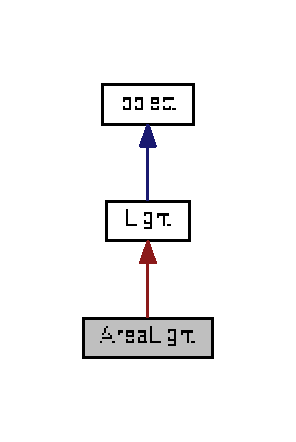
\includegraphics[width=142pt]{classAreaLight__inherit__graph}
\end{center}
\end{figure}


Collaboration diagram for Area\+Light\+:\nopagebreak
\begin{figure}[H]
\begin{center}
\leavevmode
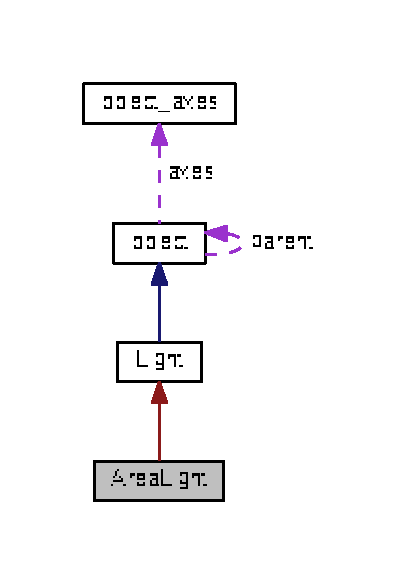
\includegraphics[width=191pt]{classAreaLight__coll__graph}
\end{center}
\end{figure}


The documentation for this class was generated from the following file\+:\begin{DoxyCompactItemize}
\item 
include/light.\+h\end{DoxyCompactItemize}

\hypertarget{classcamera}{}\section{camera Class Reference}
\label{classcamera}\index{camera@{camera}}


Inheritance diagram for camera\+:\nopagebreak
\begin{figure}[H]
\begin{center}
\leavevmode
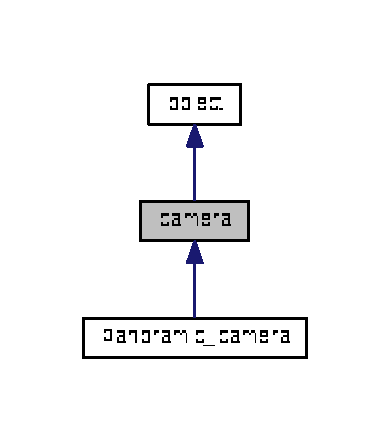
\includegraphics[width=187pt]{classcamera__inherit__graph}
\end{center}
\end{figure}


Collaboration diagram for camera\+:\nopagebreak
\begin{figure}[H]
\begin{center}
\leavevmode
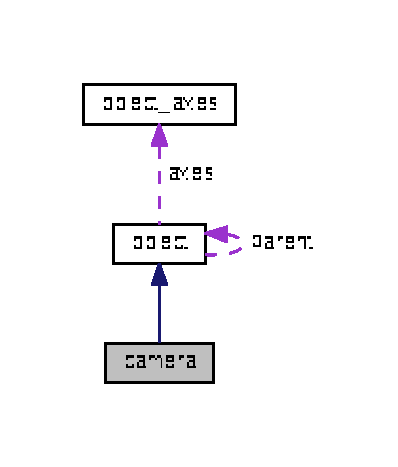
\includegraphics[width=191pt]{classcamera__coll__graph}
\end{center}
\end{figure}
\subsection*{Public Member Functions}
\begin{DoxyCompactItemize}
\item 
\mbox{\Hypertarget{classcamera_afecbb7cc19e96f75ce586aa1e11cac5a}\label{classcamera_afecbb7cc19e96f75ce586aa1e11cac5a}} 
void {\bfseries Set\+Camera\+Type} (int camera\+\_\+type)
\item 
\mbox{\Hypertarget{classcamera_a47c54b248b72d28ab8bad6469c03d25c}\label{classcamera_a47c54b248b72d28ab8bad6469c03d25c}} 
void {\bfseries Set\+Camera\+Name} (string camera\+\_\+name)
\end{DoxyCompactItemize}
\subsection*{Additional Inherited Members}


The documentation for this class was generated from the following files\+:\begin{DoxyCompactItemize}
\item 
include/camera.\+h\item 
src/camera.\+cpp\end{DoxyCompactItemize}

\hypertarget{classcone}{}\section{cone Class Reference}
\label{classcone}\index{cone@{cone}}


Inheritance diagram for cone\+:\nopagebreak
\begin{figure}[H]
\begin{center}
\leavevmode
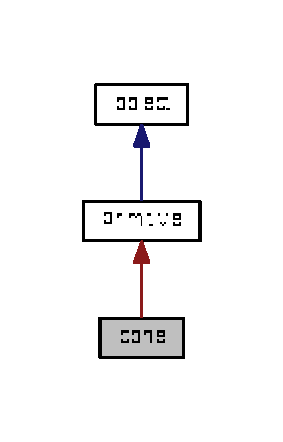
\includegraphics[width=136pt]{classcone__inherit__graph}
\end{center}
\end{figure}


Collaboration diagram for cone\+:\nopagebreak
\begin{figure}[H]
\begin{center}
\leavevmode
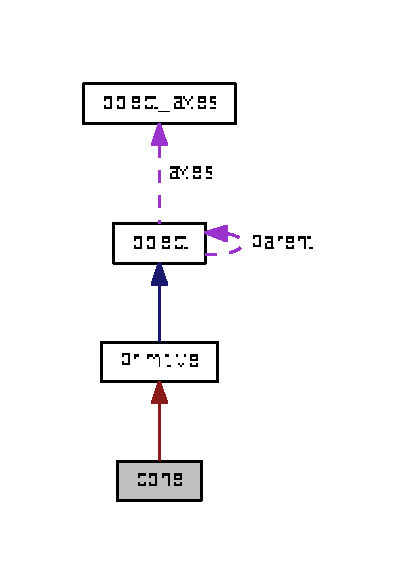
\includegraphics[width=191pt]{classcone__coll__graph}
\end{center}
\end{figure}
\subsection*{Public Member Functions}
\begin{DoxyCompactItemize}
\item 
\mbox{\Hypertarget{classcone_adabf8f53de11b1308195a662f6bc5d19}\label{classcone_adabf8f53de11b1308195a662f6bc5d19}} 
void {\bfseries make\+\_\+cone} (int horizontal\+\_\+subdiv, int vertical\+\_\+subdiv, int conic\+\_\+subdiv, int spherical\+\_\+long\+\_\+subdiv, int spherical\+\_\+lat\+\_\+subdiv, int x\+\_\+rotation, int torus\+\_\+angle, int top\+\_\+radius, int bot\+\_\+radius, int radius, int spherical\+\_\+radius, int conic\+\_\+angle, int height, int rot\+\_\+subdiv)
\end{DoxyCompactItemize}


The documentation for this class was generated from the following files\+:\begin{DoxyCompactItemize}
\item 
include/primitive.\+h\item 
src/primitive.\+cpp\end{DoxyCompactItemize}

\hypertarget{classcube}{}\section{cube Class Reference}
\label{classcube}\index{cube@{cube}}


Inheritance diagram for cube\+:\nopagebreak
\begin{figure}[H]
\begin{center}
\leavevmode
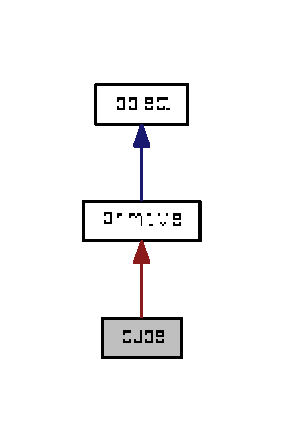
\includegraphics[width=136pt]{classcube__inherit__graph}
\end{center}
\end{figure}


Collaboration diagram for cube\+:\nopagebreak
\begin{figure}[H]
\begin{center}
\leavevmode
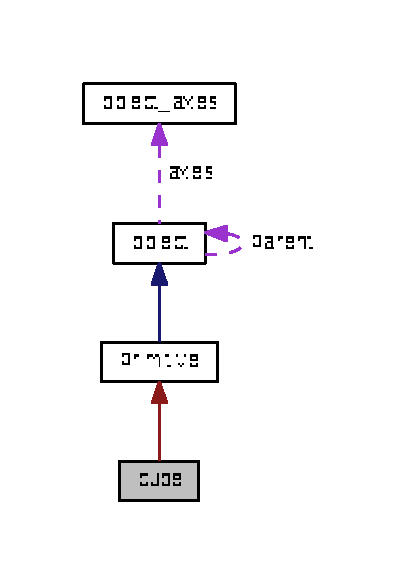
\includegraphics[width=191pt]{classcube__coll__graph}
\end{center}
\end{figure}
\subsection*{Public Member Functions}
\begin{DoxyCompactItemize}
\item 
\mbox{\Hypertarget{classcube_a2ceeae0acbecd1a5538d3ff235d4cde8}\label{classcube_a2ceeae0acbecd1a5538d3ff235d4cde8}} 
void {\bfseries make\+\_\+cube} (int horizontal\+\_\+subdiv, int vertical\+\_\+subdiv, int conic\+\_\+subdiv, int spherical\+\_\+long\+\_\+subdiv, int spherical\+\_\+lat\+\_\+subdiv, int x\+\_\+rotation, int torus\+\_\+angle, int top\+\_\+radius, int bot\+\_\+radius, int radius, int spherical\+\_\+radius, int conic\+\_\+angle, int height, int rot\+\_\+subdiv)
\end{DoxyCompactItemize}


The documentation for this class was generated from the following files\+:\begin{DoxyCompactItemize}
\item 
include/primitive.\+h\item 
src/primitive.\+cpp\end{DoxyCompactItemize}

\hypertarget{classcylinder}{}\section{cylinder Class Reference}
\label{classcylinder}\index{cylinder@{cylinder}}


Inheritance diagram for cylinder\+:\nopagebreak
\begin{figure}[H]
\begin{center}
\leavevmode
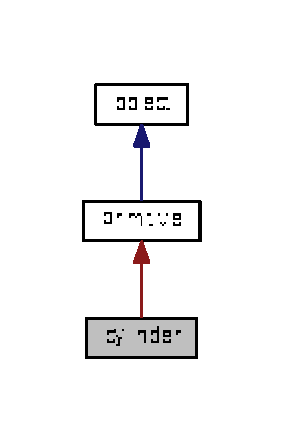
\includegraphics[width=136pt]{classcylinder__inherit__graph}
\end{center}
\end{figure}


Collaboration diagram for cylinder\+:\nopagebreak
\begin{figure}[H]
\begin{center}
\leavevmode
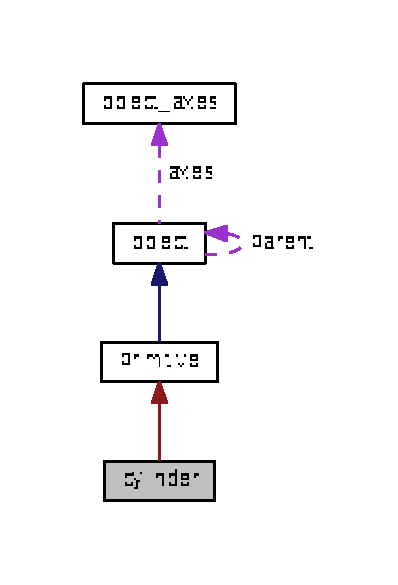
\includegraphics[width=191pt]{classcylinder__coll__graph}
\end{center}
\end{figure}
\subsection*{Public Member Functions}
\begin{DoxyCompactItemize}
\item 
\mbox{\Hypertarget{classcylinder_a31170e0b630d2210a08434e885ce76bd}\label{classcylinder_a31170e0b630d2210a08434e885ce76bd}} 
void {\bfseries make\+\_\+cylinder} (int horizontal\+\_\+subdiv, int vertical\+\_\+subdiv, int conic\+\_\+subdiv, int spherical\+\_\+long\+\_\+subdiv, int spherical\+\_\+lat\+\_\+subdiv, int x\+\_\+rotation, int torus\+\_\+angle, int top\+\_\+radius, int bot\+\_\+radius, int radius, int spherical\+\_\+radius, int conic\+\_\+angle, int height, int rot\+\_\+subdiv)
\end{DoxyCompactItemize}


The documentation for this class was generated from the following files\+:\begin{DoxyCompactItemize}
\item 
include/primitive.\+h\item 
src/primitive.\+cpp\end{DoxyCompactItemize}

\hypertarget{classdisplay}{}\section{display Class Reference}
\label{classdisplay}\index{display@{display}}
\subsection*{Public Member Functions}
\begin{DoxyCompactItemize}
\item 
\mbox{\Hypertarget{classdisplay_a4148a7a57f6a6e56008156817d9984b1}\label{classdisplay_a4148a7a57f6a6e56008156817d9984b1}} 
void {\bfseries create\+\_\+display} (int num\+\_\+displays)
\end{DoxyCompactItemize}


The documentation for this class was generated from the following file\+:\begin{DoxyCompactItemize}
\item 
include/display.\+h\end{DoxyCompactItemize}

\hypertarget{classdivider}{}\section{divider Class Reference}
\label{classdivider}\index{divider@{divider}}
\subsection*{Static Public Member Functions}
\begin{DoxyCompactItemize}
\item 
\mbox{\Hypertarget{classdivider_a0e66ef52ed97069f741241560107a8fa}\label{classdivider_a0e66ef52ed97069f741241560107a8fa}} 
static int {\bfseries divideri} (int var1, int var2)
\item 
\mbox{\Hypertarget{classdivider_a88d4fd11d1d0c14d92ca4c411dd82bc5}\label{classdivider_a88d4fd11d1d0c14d92ca4c411dd82bc5}} 
static double {\bfseries dividerd} (double var1, double var2)
\end{DoxyCompactItemize}


The documentation for this class was generated from the following file\+:\begin{DoxyCompactItemize}
\item 
include/divider.\+h\end{DoxyCompactItemize}

\hypertarget{classedge}{}\section{edge Class Reference}
\label{classedge}\index{edge@{edge}}


Collaboration diagram for edge\+:\nopagebreak
\begin{figure}[H]
\begin{center}
\leavevmode
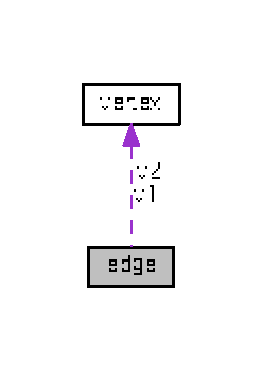
\includegraphics[width=126pt]{classedge__coll__graph}
\end{center}
\end{figure}
\subsection*{Public Member Functions}
\begin{DoxyCompactItemize}
\item 
\mbox{\Hypertarget{classedge_adad9b84c050f0205df79330003db9a8e}\label{classedge_adad9b84c050f0205df79330003db9a8e}} 
float $\ast$ {\bfseries Get\+Location} (void)
\item 
\mbox{\Hypertarget{classedge_ab446f29f3631c806e271c7146f149508}\label{classedge_ab446f29f3631c806e271c7146f149508}} 
void {\bfseries Set\+Location} (float X, float Y, float Z)
\item 
\mbox{\Hypertarget{classedge_aa04ed891daf5fa70f3ee699e555e5cef}\label{classedge_aa04ed891daf5fa70f3ee699e555e5cef}} 
float $\ast$ {\bfseries Get\+Scale} (void)
\item 
\mbox{\Hypertarget{classedge_aed961c0636e11338bdc7414cd9a3f1f5}\label{classedge_aed961c0636e11338bdc7414cd9a3f1f5}} 
void {\bfseries Set\+Scale} (float X, float Y, float Z)
\end{DoxyCompactItemize}
\subsection*{Protected Attributes}
\begin{DoxyCompactItemize}
\item 
\mbox{\Hypertarget{classedge_ae2e5280a9a1f2519d070a9ae95e2d40d}\label{classedge_ae2e5280a9a1f2519d070a9ae95e2d40d}} 
vector$<$ \hyperlink{classface}{face} $>$ {\bfseries faces}
\item 
\mbox{\Hypertarget{classedge_a0209c03c9479528b2e060d4d0e58b461}\label{classedge_a0209c03c9479528b2e060d4d0e58b461}} 
\hyperlink{classvertex}{vertex} {\bfseries v1}
\item 
\mbox{\Hypertarget{classedge_a5b849de3794f7e5126fc8f03199d568c}\label{classedge_a5b849de3794f7e5126fc8f03199d568c}} 
\hyperlink{classvertex}{vertex} {\bfseries v2}
\item 
\mbox{\Hypertarget{classedge_ab1adb65641c26fbb6b5a4f0d2d15ba6b}\label{classedge_ab1adb65641c26fbb6b5a4f0d2d15ba6b}} 
float {\bfseries location} \mbox{[}3\mbox{]}
\item 
\mbox{\Hypertarget{classedge_a7f28a6bc883fe629bbd4e90b2f5d7bdd}\label{classedge_a7f28a6bc883fe629bbd4e90b2f5d7bdd}} 
float {\bfseries scale} \mbox{[}3\mbox{]}
\end{DoxyCompactItemize}


The documentation for this class was generated from the following files\+:\begin{DoxyCompactItemize}
\item 
include/geometry.\+h\item 
src/geometry.\+cpp\end{DoxyCompactItemize}

\hypertarget{classface}{}\section{face Class Reference}
\label{classface}\index{face@{face}}
\subsection*{Public Member Functions}
\begin{DoxyCompactItemize}
\item 
\mbox{\Hypertarget{classface_a308875a2b47d0b3b53e406e1b9310a1c}\label{classface_a308875a2b47d0b3b53e406e1b9310a1c}} 
void {\bfseries Set\+Num\+Vertices} (int num\+\_\+vertices)
\item 
\mbox{\Hypertarget{classface_a345c597eb374c07b8fad51c51b5c9aba}\label{classface_a345c597eb374c07b8fad51c51b5c9aba}} 
void {\bfseries Set\+Num\+Edges} (int num\+\_\+edges)
\item 
\mbox{\Hypertarget{classface_a263f47c5a0714d2f9fb7067d24603b07}\label{classface_a263f47c5a0714d2f9fb7067d24603b07}} 
int {\bfseries Get\+Num\+Vertices} (void)
\item 
\mbox{\Hypertarget{classface_a04921ee060440a416098fd62ad8ed55d}\label{classface_a04921ee060440a416098fd62ad8ed55d}} 
int {\bfseries Get\+Num\+Edges} (void)
\item 
\mbox{\Hypertarget{classface_aed1a53fd90c464622d9ec00b70143c49}\label{classface_aed1a53fd90c464622d9ec00b70143c49}} 
void {\bfseries Set\+Location} (float X, float Y, float Z)
\item 
\mbox{\Hypertarget{classface_a699a579160b5f165bdd4d99c102d8103}\label{classface_a699a579160b5f165bdd4d99c102d8103}} 
float $\ast$ {\bfseries Get\+Location} ()
\item 
\mbox{\Hypertarget{classface_a71969f0627480de1764fcbb13de379c3}\label{classface_a71969f0627480de1764fcbb13de379c3}} 
void {\bfseries Set\+Rotation} (float X, float Y, float Z)
\item 
\mbox{\Hypertarget{classface_a9f3e71973ddda30f0cdddbc288d4e748}\label{classface_a9f3e71973ddda30f0cdddbc288d4e748}} 
float $\ast$ {\bfseries Get\+Rotation} ()
\item 
\mbox{\Hypertarget{classface_a282640bd3aabb05eb7c4a1fa1311db52}\label{classface_a282640bd3aabb05eb7c4a1fa1311db52}} 
void {\bfseries Set\+Size} (float X, float Y, float Z)
\item 
\mbox{\Hypertarget{classface_aa3971953d8cb1688e5d4cce2a466bb58}\label{classface_aa3971953d8cb1688e5d4cce2a466bb58}} 
float $\ast$ {\bfseries Get\+Size} ()
\item 
\mbox{\Hypertarget{classface_a1d191169d815678ce8969b2174359d20}\label{classface_a1d191169d815678ce8969b2174359d20}} 
void {\bfseries Add\+Vertex\+To\+Face} (\hyperlink{classvertex}{vertex})
\item 
\mbox{\Hypertarget{classface_a075797e1980d676cddc1b96e881dbd89}\label{classface_a075797e1980d676cddc1b96e881dbd89}} 
void {\bfseries Add\+Edge\+To\+Face} ()
\item 
\mbox{\Hypertarget{classface_af06f838827ab57ca07b44d6470773410}\label{classface_af06f838827ab57ca07b44d6470773410}} 
void {\bfseries Del\+Vertex\+From\+Face} (\hyperlink{classface}{face})
\item 
\mbox{\Hypertarget{classface_ac04c01fc9775f80e4f051ebd12fa13e3}\label{classface_ac04c01fc9775f80e4f051ebd12fa13e3}} 
void {\bfseries Del\+Edge\+From\+Face} (\hyperlink{classface}{face})
\end{DoxyCompactItemize}
\subsection*{Protected Attributes}
\begin{DoxyCompactItemize}
\item 
\mbox{\Hypertarget{classface_a2314e1606f18e1646e3699d216972f85}\label{classface_a2314e1606f18e1646e3699d216972f85}} 
float {\bfseries location} \mbox{[}3\mbox{]}
\item 
\mbox{\Hypertarget{classface_a985dcf85600ca0b8263140a494543cda}\label{classface_a985dcf85600ca0b8263140a494543cda}} 
float {\bfseries rotation} \mbox{[}3\mbox{]}
\item 
\mbox{\Hypertarget{classface_a9d9ac2b120c2123e95acfd75e66a8950}\label{classface_a9d9ac2b120c2123e95acfd75e66a8950}} 
float {\bfseries size} \mbox{[}3\mbox{]}
\item 
\mbox{\Hypertarget{classface_a59ed8b29c67536b39b5e7f43f674c721}\label{classface_a59ed8b29c67536b39b5e7f43f674c721}} 
int {\bfseries num\+\_\+edges}
\item 
\mbox{\Hypertarget{classface_abc378bcf2fb620c005f071c83c952fb5}\label{classface_abc378bcf2fb620c005f071c83c952fb5}} 
int {\bfseries num\+\_\+vertices}
\item 
\mbox{\Hypertarget{classface_adf25ae0e541f2fa5e9fa27cdbf6a1cb5}\label{classface_adf25ae0e541f2fa5e9fa27cdbf6a1cb5}} 
vector$<$ \hyperlink{classtexture}{texture} $>$ {\bfseries textures}
\item 
\mbox{\Hypertarget{classface_a2bcf95c5c271ade955be8db5a3a9c9ba}\label{classface_a2bcf95c5c271ade955be8db5a3a9c9ba}} 
vector$<$ \hyperlink{classvertex}{vertex} $>$ {\bfseries polygons}
\item 
\mbox{\Hypertarget{classface_a7558f66892269ccd614ebb3950336d41}\label{classface_a7558f66892269ccd614ebb3950336d41}} 
vector$<$ \hyperlink{classedge}{edge} $>$ {\bfseries edges}
\end{DoxyCompactItemize}


The documentation for this class was generated from the following files\+:\begin{DoxyCompactItemize}
\item 
include/geometry.\+h\item 
src/geometry.\+cpp\end{DoxyCompactItemize}

\hypertarget{classframe}{}\section{frame Class Reference}
\label{classframe}\index{frame@{frame}}
\subsection*{Public Member Functions}
\begin{DoxyCompactItemize}
\item 
\mbox{\Hypertarget{classframe_a14c439c71e64179c6ae6d54aee3d7598}\label{classframe_a14c439c71e64179c6ae6d54aee3d7598}} 
void {\bfseries set\+\_\+look\+\_\+at\+\_\+point} (bool look\+\_\+at\+\_\+point, int X, int Y, int Z)
\item 
\mbox{\Hypertarget{classframe_aeec2715a6e21ba2d2248eba3ec5a2cfb}\label{classframe_aeec2715a6e21ba2d2248eba3ec5a2cfb}} 
void {\bfseries unset\+\_\+look\+\_\+at\+\_\+point} (bool look\+\_\+at\+\_\+point)
\item 
\mbox{\Hypertarget{classframe_a52aa4eb0edf68e5bbf3e9a586d20ab9e}\label{classframe_a52aa4eb0edf68e5bbf3e9a586d20ab9e}} 
void {\bfseries set\+\_\+rotation} (float rotation\mbox{[}16\mbox{]})
\item 
\mbox{\Hypertarget{classframe_a0d95498d2e4f983518e9640d65c92443}\label{classframe_a0d95498d2e4f983518e9640d65c92443}} 
void {\bfseries set\+\_\+translation} (int X, int Y, int Z)
\item 
\mbox{\Hypertarget{classframe_aa8ec8d24f72722a5c6f32d549b17bd92}\label{classframe_aa8ec8d24f72722a5c6f32d549b17bd92}} 
void {\bfseries set\+\_\+scale} (int X, int Y, int Z)
\item 
\mbox{\Hypertarget{classframe_a6c1fa1eb36bb8ee0c4ce88082c278d90}\label{classframe_a6c1fa1eb36bb8ee0c4ce88082c278d90}} 
float $\ast$ {\bfseries get\+\_\+rotate} (void)
\item 
\mbox{\Hypertarget{classframe_a2438d34d2e8523d8fdbbaefd52d37e3f}\label{classframe_a2438d34d2e8523d8fdbbaefd52d37e3f}} 
float $\ast$ {\bfseries get\+\_\+translate} (void)
\item 
\mbox{\Hypertarget{classframe_a28904818d025cfe902ed0956b8fe7f9b}\label{classframe_a28904818d025cfe902ed0956b8fe7f9b}} 
float $\ast$ {\bfseries get\+\_\+scale} (void)
\end{DoxyCompactItemize}
\subsection*{Public Attributes}
\begin{DoxyCompactItemize}
\item 
\mbox{\Hypertarget{classframe_a5dcc3ab35351bca7bfd3f2fe916f1651}\label{classframe_a5dcc3ab35351bca7bfd3f2fe916f1651}} 
bool {\bfseries is\+\_\+keyframe}
\item 
\mbox{\Hypertarget{classframe_abcc53e8268c089969571888bfb2c9ed3}\label{classframe_abcc53e8268c089969571888bfb2c9ed3}} 
float {\bfseries rotate} \mbox{[}16\mbox{]} = \{ 0.\+0, 0.\+0, 0.\+0, 0.\+0, 0.\+0, 0.\+0, 0.\+0, 0.\+0, 0.\+0, 0.\+0, 0.\+0, 0.\+0, 0.\+0, 0.\+0, 0.\+0, 0.\+0 \}
\item 
\mbox{\Hypertarget{classframe_a041ae59b3f0e599c524c6006e4f46093}\label{classframe_a041ae59b3f0e599c524c6006e4f46093}} 
float {\bfseries translate} \mbox{[}3\mbox{]} = \{ 0.\+0, 0.\+0, 0.\+0 \}
\item 
\mbox{\Hypertarget{classframe_aaea81e25dd66cb95c464e0dfe83069d2}\label{classframe_aaea81e25dd66cb95c464e0dfe83069d2}} 
float {\bfseries scale} \mbox{[}3\mbox{]} = \{ 0.\+0, 0.\+0, 0.\+0 \}
\item 
\mbox{\Hypertarget{classframe_a5b0f199fee2c096ea2af30820d57884a}\label{classframe_a5b0f199fee2c096ea2af30820d57884a}} 
bool {\bfseries look\+\_\+at\+\_\+point} = false
\item 
\mbox{\Hypertarget{classframe_ac3dd45b414b08e16fb8aa7e6128367d6}\label{classframe_ac3dd45b414b08e16fb8aa7e6128367d6}} 
float {\bfseries lookat} \mbox{[}3\mbox{]} = \{ 0.\+0, 0.\+0, 0.\+0 \}
\end{DoxyCompactItemize}


The documentation for this class was generated from the following files\+:\begin{DoxyCompactItemize}
\item 
include/animation.\+h\item 
src/animation.\+cpp\end{DoxyCompactItemize}

\hypertarget{classgeosphere}{}\section{geosphere Class Reference}
\label{classgeosphere}\index{geosphere@{geosphere}}


Inheritance diagram for geosphere\+:\nopagebreak
\begin{figure}[H]
\begin{center}
\leavevmode
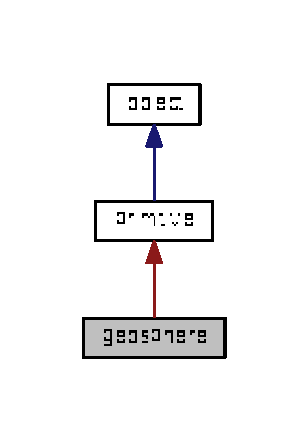
\includegraphics[width=148pt]{classgeosphere__inherit__graph}
\end{center}
\end{figure}


Collaboration diagram for geosphere\+:\nopagebreak
\begin{figure}[H]
\begin{center}
\leavevmode
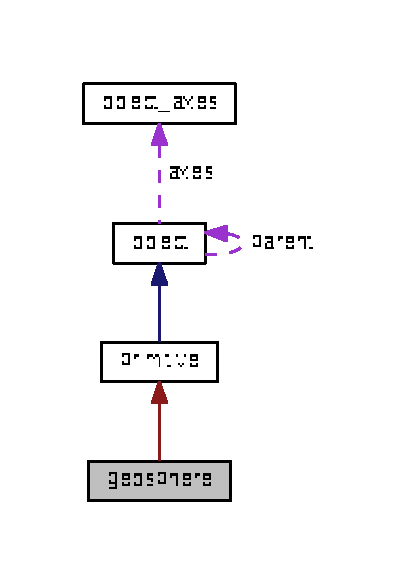
\includegraphics[width=191pt]{classgeosphere__coll__graph}
\end{center}
\end{figure}
\subsection*{Public Member Functions}
\begin{DoxyCompactItemize}
\item 
\mbox{\Hypertarget{classgeosphere_ab78c5d35e8dae24a2c5916050746151f}\label{classgeosphere_ab78c5d35e8dae24a2c5916050746151f}} 
void {\bfseries make\+\_\+geosphere} (int resolution)
\end{DoxyCompactItemize}


The documentation for this class was generated from the following files\+:\begin{DoxyCompactItemize}
\item 
include/primitive.\+h\item 
src/primitive.\+cpp\end{DoxyCompactItemize}

\hypertarget{classGoniometricLight}{}\section{Goniometric\+Light Class Reference}
\label{classGoniometricLight}\index{Goniometric\+Light@{Goniometric\+Light}}


Inheritance diagram for Goniometric\+Light\+:\nopagebreak
\begin{figure}[H]
\begin{center}
\leavevmode
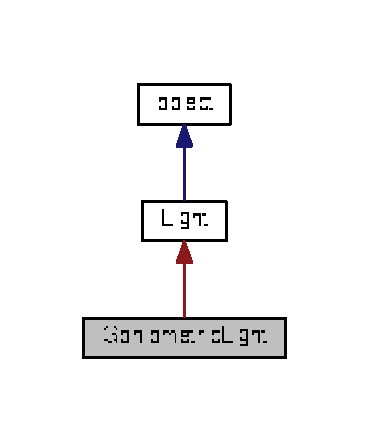
\includegraphics[width=177pt]{classGoniometricLight__inherit__graph}
\end{center}
\end{figure}


Collaboration diagram for Goniometric\+Light\+:\nopagebreak
\begin{figure}[H]
\begin{center}
\leavevmode
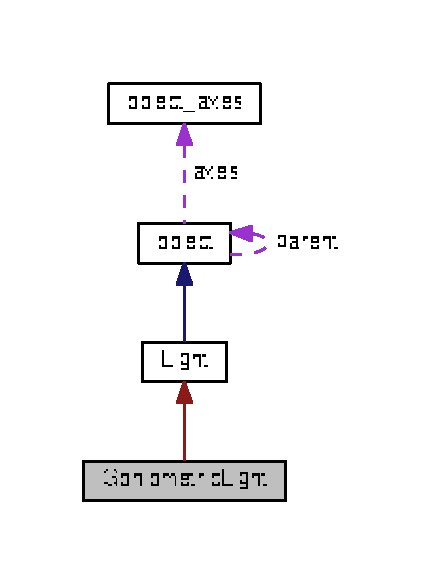
\includegraphics[width=203pt]{classGoniometricLight__coll__graph}
\end{center}
\end{figure}


The documentation for this class was generated from the following file\+:\begin{DoxyCompactItemize}
\item 
include/light.\+h\end{DoxyCompactItemize}

\hypertarget{classgui}{}\section{gui Class Reference}
\label{classgui}\index{gui@{gui}}


Inheritance diagram for gui\+:\nopagebreak
\begin{figure}[H]
\begin{center}
\leavevmode
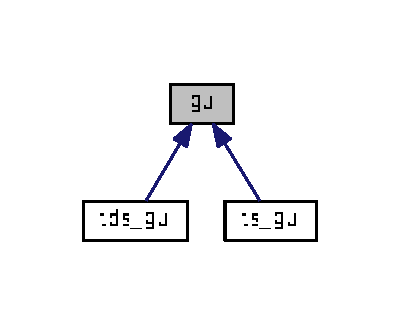
\includegraphics[width=192pt]{classgui__inherit__graph}
\end{center}
\end{figure}
\subsection*{Public Member Functions}
\begin{DoxyCompactItemize}
\item 
\mbox{\Hypertarget{classgui_a1a5906415ded816116a23822bd73b5f1}\label{classgui_a1a5906415ded816116a23822bd73b5f1}} 
void {\bfseries make\+\_\+gui} (\hyperlink{classpreferences}{preferences} \&prefs, \hyperlink{classscene}{scene} \&\hyperlink{classscene}{scene})
\item 
\mbox{\Hypertarget{classgui_a6210811d6e2a5db2cf1548958a37dec0}\label{classgui_a6210811d6e2a5db2cf1548958a37dec0}} 
void {\bfseries setbuilder} (string)
\item 
\mbox{\Hypertarget{classgui_a4caa9c72cc2853eb33900ac74a0668ea}\label{classgui_a4caa9c72cc2853eb33900ac74a0668ea}} 
void {\bfseries setlocation} (float X, float Y, float Z)
\item 
\mbox{\Hypertarget{classgui_a43f6b66a4b1e8413bc28acd61302220a}\label{classgui_a43f6b66a4b1e8413bc28acd61302220a}} 
void {\bfseries setrotation} (float X, float Y, float Z)
\item 
\mbox{\Hypertarget{classgui_a47621e87cba0dd748d224a50dfff8673}\label{classgui_a47621e87cba0dd748d224a50dfff8673}} 
void {\bfseries setscale} (float X, float Y, float Z)
\item 
\mbox{\Hypertarget{classgui_afd6c47114356e9a7954687b5dc3297f4}\label{classgui_afd6c47114356e9a7954687b5dc3297f4}} 
float $\ast$ {\bfseries getlocation} (void)
\item 
\mbox{\Hypertarget{classgui_a4c57f420b452008a9972402555ed33ea}\label{classgui_a4c57f420b452008a9972402555ed33ea}} 
float $\ast$ {\bfseries getrotation} (void)
\item 
\mbox{\Hypertarget{classgui_a405ae67b3bc3a608c0dcf6dbe65139e8}\label{classgui_a405ae67b3bc3a608c0dcf6dbe65139e8}} 
float $\ast$ {\bfseries getscale} (void)
\item 
\mbox{\Hypertarget{classgui_a6b85b911cd3f2c6b71db91c4f07992bf}\label{classgui_a6b85b911cd3f2c6b71db91c4f07992bf}} 
int {\bfseries quit} (void)
\end{DoxyCompactItemize}
\subsection*{Protected Attributes}
\begin{DoxyCompactItemize}
\item 
\mbox{\Hypertarget{classgui_a90ebd6966fcffb39facd354ad9c9a16b}\label{classgui_a90ebd6966fcffb39facd354ad9c9a16b}} 
float {\bfseries location} \mbox{[}3\mbox{]}
\item 
\mbox{\Hypertarget{classgui_aa61d2bc7fd54ebb5b470a55c343bb36f}\label{classgui_aa61d2bc7fd54ebb5b470a55c343bb36f}} 
float {\bfseries rotation} \mbox{[}3\mbox{]}
\item 
\mbox{\Hypertarget{classgui_a718fac860741e34b56ae2a72e6df6247}\label{classgui_a718fac860741e34b56ae2a72e6df6247}} 
float {\bfseries scale} \mbox{[}3\mbox{]}
\item 
\mbox{\Hypertarget{classgui_a353888f26390a86d177ab6f91e7c6b7c}\label{classgui_a353888f26390a86d177ab6f91e7c6b7c}} 
Glib\+::\+Ref\+Ptr$<$ Gtk\+::\+Builder $>$ {\bfseries builder}
\item 
\mbox{\Hypertarget{classgui_accb3e611ba2ebd4b4747ade98473e9ba}\label{classgui_accb3e611ba2ebd4b4747ade98473e9ba}} 
Glib\+::\+Ref\+Ptr$<$ Gtk\+::\+Application $>$ {\bfseries app} = Gtk\+::\+Application\+::create(\char`\"{}M\+G2modeller++\char`\"{})
\end{DoxyCompactItemize}


The documentation for this class was generated from the following files\+:\begin{DoxyCompactItemize}
\item 
include/gui.\+h\item 
src/gui.\+cpp\end{DoxyCompactItemize}

\hypertarget{classhorizontal__text}{}\section{horizontal\+\_\+text Class Reference}
\label{classhorizontal__text}\index{horizontal\+\_\+text@{horizontal\+\_\+text}}


Inheritance diagram for horizontal\+\_\+text\+:
\nopagebreak
\begin{figure}[H]
\begin{center}
\leavevmode
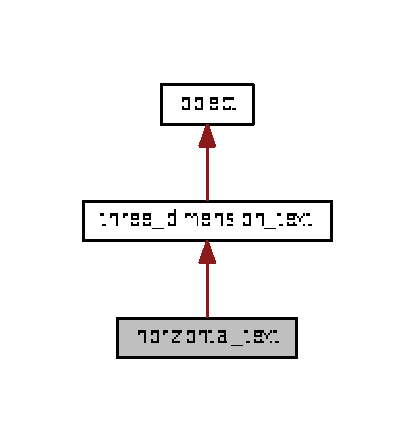
\includegraphics[width=199pt]{classhorizontal__text__inherit__graph}
\end{center}
\end{figure}


Collaboration diagram for horizontal\+\_\+text\+:
\nopagebreak
\begin{figure}[H]
\begin{center}
\leavevmode
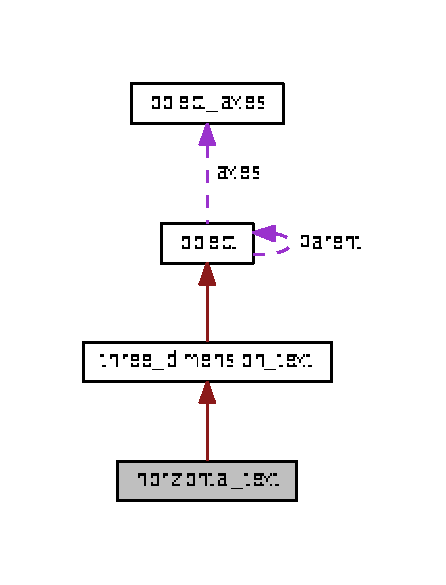
\includegraphics[width=214pt]{classhorizontal__text__coll__graph}
\end{center}
\end{figure}


The documentation for this class was generated from the following file\+:\begin{DoxyCompactItemize}
\item 
include/text.\+h\end{DoxyCompactItemize}

\hypertarget{classImageLight}{}\section{Image\+Light Class Reference}
\label{classImageLight}\index{Image\+Light@{Image\+Light}}


Inheritance diagram for Image\+Light\+:\nopagebreak
\begin{figure}[H]
\begin{center}
\leavevmode
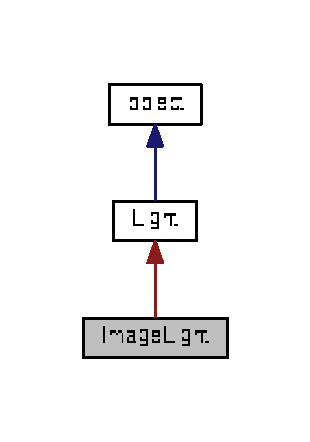
\includegraphics[width=149pt]{classImageLight__inherit__graph}
\end{center}
\end{figure}


Collaboration diagram for Image\+Light\+:\nopagebreak
\begin{figure}[H]
\begin{center}
\leavevmode
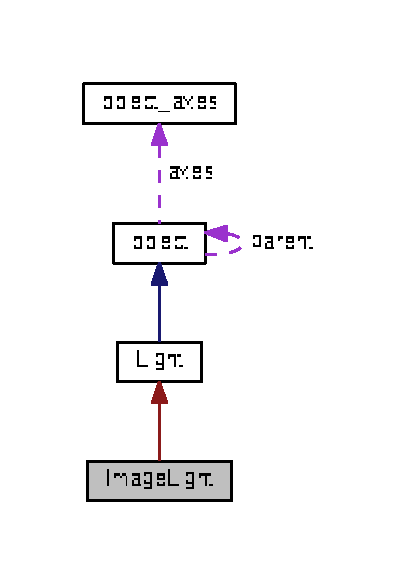
\includegraphics[width=191pt]{classImageLight__coll__graph}
\end{center}
\end{figure}


The documentation for this class was generated from the following file\+:\begin{DoxyCompactItemize}
\item 
include/light.\+h\end{DoxyCompactItemize}

\hypertarget{classInfiniteLight}{}\section{Infinite\+Light Class Reference}
\label{classInfiniteLight}\index{Infinite\+Light@{Infinite\+Light}}


Inheritance diagram for Infinite\+Light\+:\nopagebreak
\begin{figure}[H]
\begin{center}
\leavevmode
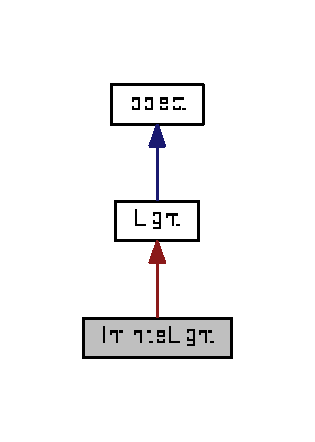
\includegraphics[width=151pt]{classInfiniteLight__inherit__graph}
\end{center}
\end{figure}


Collaboration diagram for Infinite\+Light\+:\nopagebreak
\begin{figure}[H]
\begin{center}
\leavevmode
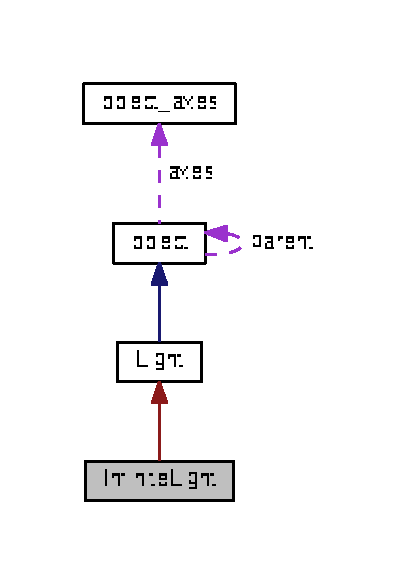
\includegraphics[width=191pt]{classInfiniteLight__coll__graph}
\end{center}
\end{figure}


The documentation for this class was generated from the following file\+:\begin{DoxyCompactItemize}
\item 
include/light.\+h\end{DoxyCompactItemize}

\hypertarget{classLight}{}\section{Light Class Reference}
\label{classLight}\index{Light@{Light}}


Inheritance diagram for Light\+:\nopagebreak
\begin{figure}[H]
\begin{center}
\leavevmode
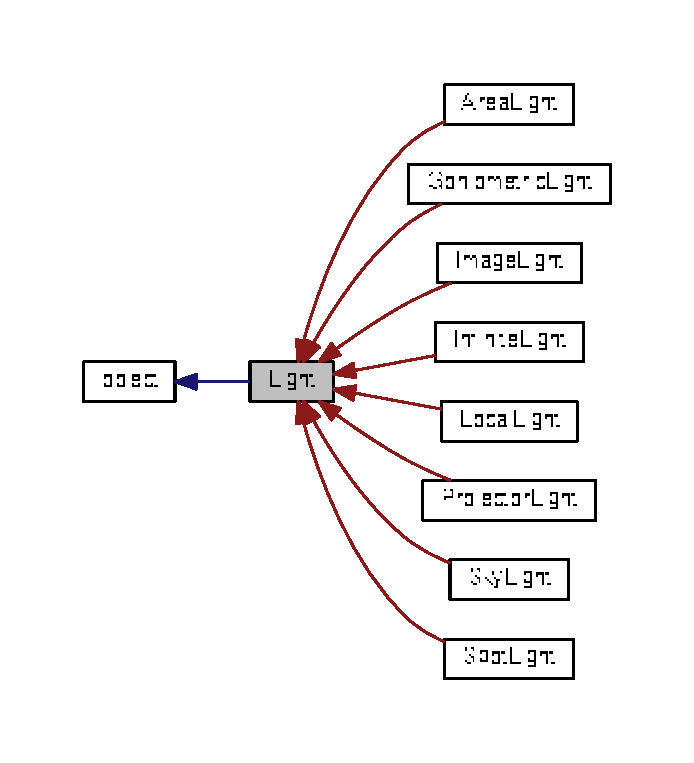
\includegraphics[width=333pt]{classLight__inherit__graph}
\end{center}
\end{figure}


Collaboration diagram for Light\+:\nopagebreak
\begin{figure}[H]
\begin{center}
\leavevmode
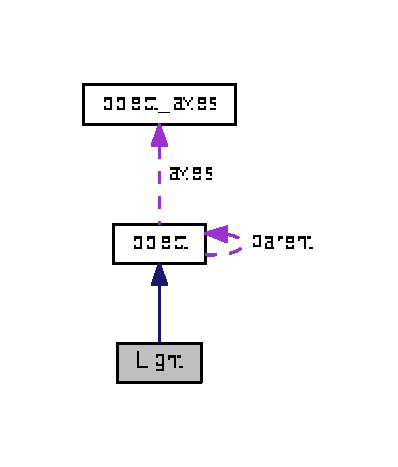
\includegraphics[width=191pt]{classLight__coll__graph}
\end{center}
\end{figure}
\subsection*{Protected Attributes}
\begin{DoxyCompactItemize}
\item 
\mbox{\Hypertarget{classLight_a54cfb73518034aede0953e3098613928}\label{classLight_a54cfb73518034aede0953e3098613928}} 
int {\bfseries light\+\_\+type}
\item 
\mbox{\Hypertarget{classLight_a4f195d55c72f7419de6a84beabacd7d8}\label{classLight_a4f195d55c72f7419de6a84beabacd7d8}} 
double {\bfseries color} \mbox{[}3\mbox{]}
\end{DoxyCompactItemize}
\subsection*{Additional Inherited Members}


The documentation for this class was generated from the following file\+:\begin{DoxyCompactItemize}
\item 
include/light.\+h\end{DoxyCompactItemize}

\hypertarget{classLocalLight}{}\section{Local\+Light Class Reference}
\label{classLocalLight}\index{Local\+Light@{Local\+Light}}


Inheritance diagram for Local\+Light\+:\nopagebreak
\begin{figure}[H]
\begin{center}
\leavevmode
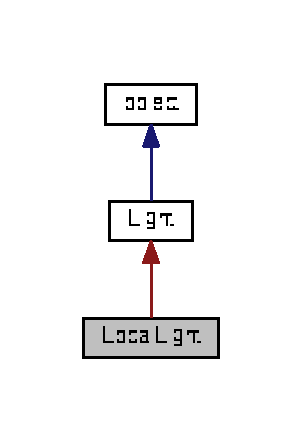
\includegraphics[width=145pt]{classLocalLight__inherit__graph}
\end{center}
\end{figure}


Collaboration diagram for Local\+Light\+:\nopagebreak
\begin{figure}[H]
\begin{center}
\leavevmode
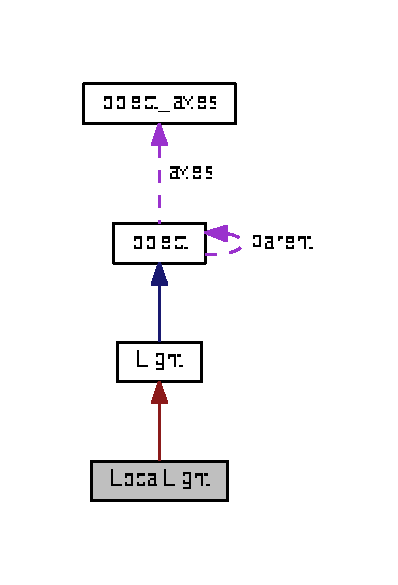
\includegraphics[width=191pt]{classLocalLight__coll__graph}
\end{center}
\end{figure}


The documentation for this class was generated from the following file\+:\begin{DoxyCompactItemize}
\item 
include/light.\+h\end{DoxyCompactItemize}

\hypertarget{classmaterial}{}\section{material Class Reference}
\label{classmaterial}\index{material@{material}}
\subsection*{Public Member Functions}
\begin{DoxyCompactItemize}
\item 
\mbox{\Hypertarget{classmaterial_a2e0c23b3aa942192e63ecfcef6d6cc3a}\label{classmaterial_a2e0c23b3aa942192e63ecfcef6d6cc3a}} 
void {\bfseries set\+\_\+use\+\_\+image} (bool use\+\_\+image)
\item 
\mbox{\Hypertarget{classmaterial_a19ad600f4e34c7c8a54c2ae4ad2686ff}\label{classmaterial_a19ad600f4e34c7c8a54c2ae4ad2686ff}} 
void {\bfseries set\+\_\+image} (string image)
\item 
\mbox{\Hypertarget{classmaterial_aeda1f81477e9014cc249aa1704e61e76}\label{classmaterial_aeda1f81477e9014cc249aa1704e61e76}} 
void {\bfseries set\+\_\+image\+\_\+\+U\+\_\+repeats} (float u\+\_\+repeats)
\item 
\mbox{\Hypertarget{classmaterial_a6e15ddcbb959d94ad018c2974ac7c67d}\label{classmaterial_a6e15ddcbb959d94ad018c2974ac7c67d}} 
void {\bfseries set\+\_\+image\+\_\+\+V\+\_\+repeats} (float u\+\_\+repeats)
\item 
\mbox{\Hypertarget{classmaterial_a0cb4282457e38af015b338900ee03e2c}\label{classmaterial_a0cb4282457e38af015b338900ee03e2c}} 
void {\bfseries set\+\_\+image\+\_\+\+U\+\_\+offset} (float u\+\_\+offset)
\item 
\mbox{\Hypertarget{classmaterial_aae382b5ac81ab34e173f3cec36748cf8}\label{classmaterial_aae382b5ac81ab34e173f3cec36748cf8}} 
void {\bfseries set\+\_\+image\+\_\+\+V\+\_\+offset} (float u\+\_\+offset)
\item 
\mbox{\Hypertarget{classmaterial_a318adce5597355d2c527c18b6f84a2e5}\label{classmaterial_a318adce5597355d2c527c18b6f84a2e5}} 
void {\bfseries set\+\_\+color} (int R, int G, int B)
\item 
\mbox{\Hypertarget{classmaterial_a0f5c19149139579cb56fadd9f9736d4b}\label{classmaterial_a0f5c19149139579cb56fadd9f9736d4b}} 
void {\bfseries set\+\_\+use\+\_\+transparency} (bool use\+\_\+trans)
\item 
\mbox{\Hypertarget{classmaterial_a0dd22e29b2d0614f0a71df555d7c58a4}\label{classmaterial_a0dd22e29b2d0614f0a71df555d7c58a4}} 
void {\bfseries set\+\_\+use\+\_\+transparency\+\_\+map} (bool use\+\_\+trans\+\_\+map)
\item 
\mbox{\Hypertarget{classmaterial_a5070c6cd92644fd8787b623bf9b44684}\label{classmaterial_a5070c6cd92644fd8787b623bf9b44684}} 
void {\bfseries set\+\_\+transparency\+\_\+map} (string trans\+\_\+map)
\item 
\mbox{\Hypertarget{classmaterial_a044c25a67ce59ed29a24f9528c001bd8}\label{classmaterial_a044c25a67ce59ed29a24f9528c001bd8}} 
void {\bfseries set\+\_\+trans\+\_\+map\+\_\+\+U\+\_\+repeats} (float trans\+\_\+map\+\_\+\+U\+\_\+repeats)
\item 
\mbox{\Hypertarget{classmaterial_a2f2338b6253d29ec85b383502b3f2459}\label{classmaterial_a2f2338b6253d29ec85b383502b3f2459}} 
void {\bfseries set\+\_\+trans\+\_\+map\+\_\+\+V\+\_\+repeats} (float trans\+\_\+map\+\_\+\+V\+\_\+repeats)
\item 
\mbox{\Hypertarget{classmaterial_a6c6d3125fca60347fcda6e743d2302ac}\label{classmaterial_a6c6d3125fca60347fcda6e743d2302ac}} 
void {\bfseries set\+\_\+trans\+\_\+map\+\_\+\+U\+\_\+offset} (float trans\+\_\+map\+\_\+\+U\+\_\+offset)
\item 
\mbox{\Hypertarget{classmaterial_a1ca6ee1f3dfb734f87fc535b1af8a710}\label{classmaterial_a1ca6ee1f3dfb734f87fc535b1af8a710}} 
void {\bfseries set\+\_\+trans\+\_\+map\+\_\+\+V\+\_\+offset} (float trans\+\_\+map\+\_\+\+V\+\_\+offset)
\item 
\mbox{\Hypertarget{classmaterial_a5ad7f22b608d724c7a69f735737831d8}\label{classmaterial_a5ad7f22b608d724c7a69f735737831d8}} 
void {\bfseries set\+\_\+use\+\_\+bump} (bool)
\item 
\mbox{\Hypertarget{classmaterial_a090fec60f7f42081f671addb8ab1b8b9}\label{classmaterial_a090fec60f7f42081f671addb8ab1b8b9}} 
void {\bfseries set\+\_\+bump} (string)
\item 
\mbox{\Hypertarget{classmaterial_a99d19756c96e2e4f9602a5dea9fa7ede}\label{classmaterial_a99d19756c96e2e4f9602a5dea9fa7ede}} 
void {\bfseries set\+\_\+luminance} (int lum)
\item 
\mbox{\Hypertarget{classmaterial_a074beebc9fc4ebe20574215398086ee9}\label{classmaterial_a074beebc9fc4ebe20574215398086ee9}} 
void {\bfseries set\+\_\+diffusion} (int diff)
\item 
\mbox{\Hypertarget{classmaterial_ae39ead64325f5877bb5b71c60d0110ea}\label{classmaterial_ae39ead64325f5877bb5b71c60d0110ea}} 
void {\bfseries set\+\_\+shininess} (int shin)
\item 
\mbox{\Hypertarget{classmaterial_ad963c73d469c2811a56e5cf99e04b71e}\label{classmaterial_ad963c73d469c2811a56e5cf99e04b71e}} 
void {\bfseries set\+\_\+specular} (int spec)
\item 
\mbox{\Hypertarget{classmaterial_a19f2f98c71689d85dcf297bb677db1a5}\label{classmaterial_a19f2f98c71689d85dcf297bb677db1a5}} 
void {\bfseries set\+\_\+specular\+\_\+color} (int R, int G, int B)
\item 
\mbox{\Hypertarget{classmaterial_ac45022ebbbd5be3b2d4a612217ffec78}\label{classmaterial_ac45022ebbbd5be3b2d4a612217ffec78}} 
void {\bfseries set\+\_\+use\+\_\+material\+\_\+light} (bool)
\item 
\mbox{\Hypertarget{classmaterial_ac8ec53ce926e139973f8933a1aa81709}\label{classmaterial_ac8ec53ce926e139973f8933a1aa81709}} 
void {\bfseries set\+\_\+intensity} (int)
\item 
\mbox{\Hypertarget{classmaterial_ae29f0fb86dc9855447bbfcaae81d4c6f}\label{classmaterial_ae29f0fb86dc9855447bbfcaae81d4c6f}} 
void {\bfseries set\+\_\+cast\+\_\+shadow} (bool)
\item 
\mbox{\Hypertarget{classmaterial_a41c83f8ef4e755606c5e3579d3196c9a}\label{classmaterial_a41c83f8ef4e755606c5e3579d3196c9a}} 
void {\bfseries set\+\_\+shadow\+\_\+transparency} (bool)
\item 
\mbox{\Hypertarget{classmaterial_a0977543e8d883234536019e5914f8a37}\label{classmaterial_a0977543e8d883234536019e5914f8a37}} 
void {\bfseries set\+\_\+shadow\+\_\+min} (float)
\item 
\mbox{\Hypertarget{classmaterial_a6ccf1dd96ee39e57eebe43363df9268a}\label{classmaterial_a6ccf1dd96ee39e57eebe43363df9268a}} 
void {\bfseries set\+\_\+shadow\+\_\+max} (float)
\end{DoxyCompactItemize}
\subsection*{Protected Attributes}
\begin{DoxyCompactItemize}
\item 
\mbox{\Hypertarget{classmaterial_a62cd5c71d10fc79149e52d380a92832f}\label{classmaterial_a62cd5c71d10fc79149e52d380a92832f}} 
bool {\bfseries use\+\_\+image} = false
\item 
\mbox{\Hypertarget{classmaterial_a9b88ba5477ecce6dedc304aa2e9c0377}\label{classmaterial_a9b88ba5477ecce6dedc304aa2e9c0377}} 
string {\bfseries image}
\item 
\mbox{\Hypertarget{classmaterial_a4b0e3e365c52f26b77bb1f4a8bf9fc75}\label{classmaterial_a4b0e3e365c52f26b77bb1f4a8bf9fc75}} 
float {\bfseries image\+\_\+\+U\+\_\+repeats} = 1.\+00
\item 
\mbox{\Hypertarget{classmaterial_ac465af4c697700bcac437dcfb1c95000}\label{classmaterial_ac465af4c697700bcac437dcfb1c95000}} 
float {\bfseries image\+\_\+\+V\+\_\+repeats} = 1.\+00
\item 
\mbox{\Hypertarget{classmaterial_a1f7f477c64806949f2aa55cbaa3c23bc}\label{classmaterial_a1f7f477c64806949f2aa55cbaa3c23bc}} 
float {\bfseries image\+\_\+\+U\+\_\+offset} = 1.\+00
\item 
\mbox{\Hypertarget{classmaterial_aa2af2c634b652eae81e726727a65199f}\label{classmaterial_aa2af2c634b652eae81e726727a65199f}} 
float {\bfseries image\+\_\+\+V\+\_\+offset} = 1.\+00
\item 
\mbox{\Hypertarget{classmaterial_aad9ca45a749b3ce86eb9d23fcc055817}\label{classmaterial_aad9ca45a749b3ce86eb9d23fcc055817}} 
int {\bfseries color} \mbox{[}3\mbox{]} = \{ 255, 255, 255 \}
\item 
\mbox{\Hypertarget{classmaterial_a1c6a200137f056eb06153667292c5649}\label{classmaterial_a1c6a200137f056eb06153667292c5649}} 
bool {\bfseries use\+\_\+transparency} = false
\item 
\mbox{\Hypertarget{classmaterial_a013b5d251a31ac28924b03d34c786ca5}\label{classmaterial_a013b5d251a31ac28924b03d34c786ca5}} 
bool {\bfseries use\+\_\+transparency\+\_\+map} = false
\item 
\mbox{\Hypertarget{classmaterial_a744c40c8110bbcfa64d5dd0a0a83fb9a}\label{classmaterial_a744c40c8110bbcfa64d5dd0a0a83fb9a}} 
string {\bfseries transparency\+\_\+map}
\item 
\mbox{\Hypertarget{classmaterial_a8751cabfd1519e436b84247a985dad44}\label{classmaterial_a8751cabfd1519e436b84247a985dad44}} 
float {\bfseries trans\+\_\+map\+\_\+\+U\+\_\+repeats} = 1.\+00
\item 
\mbox{\Hypertarget{classmaterial_a14a2abe6b059b113689cb75f652222c8}\label{classmaterial_a14a2abe6b059b113689cb75f652222c8}} 
float {\bfseries trans\+\_\+map\+\_\+\+V\+\_\+repeats} = 1.\+00
\item 
\mbox{\Hypertarget{classmaterial_a72c7e0db201e914d861caec0be4c3e8e}\label{classmaterial_a72c7e0db201e914d861caec0be4c3e8e}} 
float {\bfseries trans\+\_\+map\+\_\+\+U\+\_\+offset} = 1.\+00
\item 
\mbox{\Hypertarget{classmaterial_ad6cf1cf5fc8c617e86c4d66ce5995ff8}\label{classmaterial_ad6cf1cf5fc8c617e86c4d66ce5995ff8}} 
float {\bfseries trans\+\_\+map\+\_\+\+V\+\_\+offset} = 1.\+00
\item 
\mbox{\Hypertarget{classmaterial_ac2f9f9bcfe2328041528ef6322b59c71}\label{classmaterial_ac2f9f9bcfe2328041528ef6322b59c71}} 
bool {\bfseries use\+\_\+bump} = false
\item 
\mbox{\Hypertarget{classmaterial_ae83e4a5d834b78b59a38db6d96fba982}\label{classmaterial_ae83e4a5d834b78b59a38db6d96fba982}} 
string {\bfseries bump}
\item 
\mbox{\Hypertarget{classmaterial_a8bccc78ba19a32957f91f28322e10496}\label{classmaterial_a8bccc78ba19a32957f91f28322e10496}} 
int {\bfseries luminance} = 0
\item 
\mbox{\Hypertarget{classmaterial_adaa4ae42328332fd6bb34fe468416496}\label{classmaterial_adaa4ae42328332fd6bb34fe468416496}} 
int {\bfseries diffusion} = 100
\item 
\mbox{\Hypertarget{classmaterial_a08f6c477c078af3687d24fc446de6f24}\label{classmaterial_a08f6c477c078af3687d24fc446de6f24}} 
int {\bfseries shininess} = 0
\item 
\mbox{\Hypertarget{classmaterial_a7e30e943dc2ee28c8652dfb892144631}\label{classmaterial_a7e30e943dc2ee28c8652dfb892144631}} 
int {\bfseries specular} = 0
\item 
\mbox{\Hypertarget{classmaterial_a0e0e985fe11f12467dc84eb7e774e1ae}\label{classmaterial_a0e0e985fe11f12467dc84eb7e774e1ae}} 
int {\bfseries specular\+\_\+color} \mbox{[}3\mbox{]} = \{ 255, 255, 255 \}
\item 
\mbox{\Hypertarget{classmaterial_a0fee3e4a752a99f5205348c3c5ed9e34}\label{classmaterial_a0fee3e4a752a99f5205348c3c5ed9e34}} 
bool {\bfseries use\+\_\+material\+\_\+light} = false
\item 
\mbox{\Hypertarget{classmaterial_aa1f2a51ab9d0850560850748a261e812}\label{classmaterial_aa1f2a51ab9d0850560850748a261e812}} 
int {\bfseries intensity} = 50
\item 
\mbox{\Hypertarget{classmaterial_aafeb36f836908481e64464807dba6a63}\label{classmaterial_aafeb36f836908481e64464807dba6a63}} 
bool {\bfseries cast\+\_\+shadow} = false
\item 
\mbox{\Hypertarget{classmaterial_a011488b6f2999635cd62d61e1edb109b}\label{classmaterial_a011488b6f2999635cd62d61e1edb109b}} 
bool {\bfseries shadow\+\_\+transparency} = false
\item 
\mbox{\Hypertarget{classmaterial_a1570607560ba31306b12323aa928f92e}\label{classmaterial_a1570607560ba31306b12323aa928f92e}} 
float {\bfseries min} = 0.\+50
\item 
\mbox{\Hypertarget{classmaterial_aee71636124c85fe10d6f53e003ef247b}\label{classmaterial_aee71636124c85fe10d6f53e003ef247b}} 
float {\bfseries max} = 0.\+10
\end{DoxyCompactItemize}


The documentation for this class was generated from the following file\+:\begin{DoxyCompactItemize}
\item 
include/material.\+h\end{DoxyCompactItemize}

\hypertarget{classmetaball}{}\section{metaball Class Reference}
\label{classmetaball}\index{metaball@{metaball}}


Inheritance diagram for metaball\+:\nopagebreak
\begin{figure}[H]
\begin{center}
\leavevmode
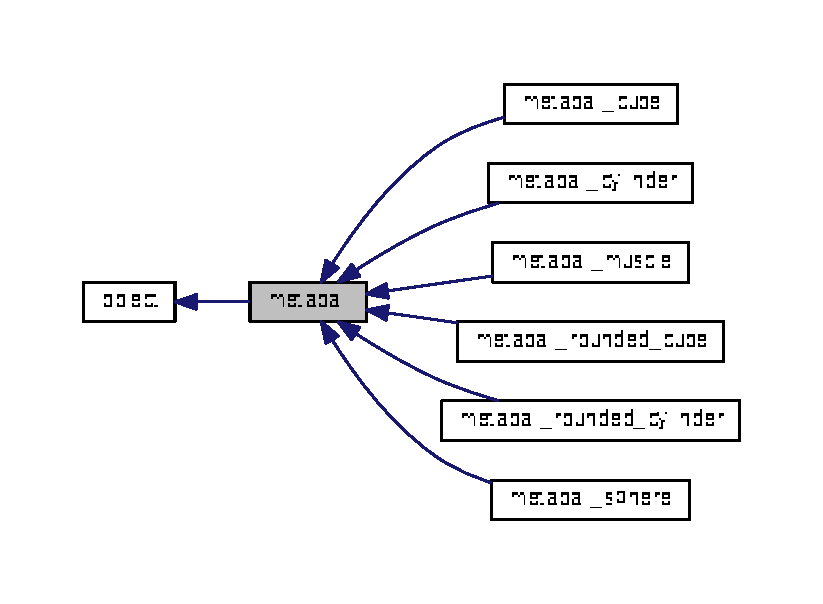
\includegraphics[width=350pt]{classmetaball__inherit__graph}
\end{center}
\end{figure}


Collaboration diagram for metaball\+:\nopagebreak
\begin{figure}[H]
\begin{center}
\leavevmode
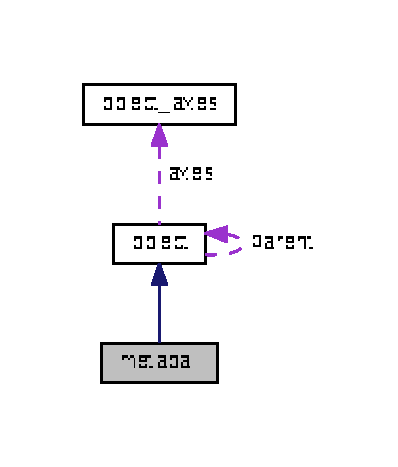
\includegraphics[width=191pt]{classmetaball__coll__graph}
\end{center}
\end{figure}
\subsection*{Additional Inherited Members}


The documentation for this class was generated from the following file\+:\begin{DoxyCompactItemize}
\item 
include/metaball.\+h\end{DoxyCompactItemize}

\hypertarget{classmetaball__cube}{}\section{metaball\+\_\+cube Class Reference}
\label{classmetaball__cube}\index{metaball\+\_\+cube@{metaball\+\_\+cube}}


Inheritance diagram for metaball\+\_\+cube\+:\nopagebreak
\begin{figure}[H]
\begin{center}
\leavevmode
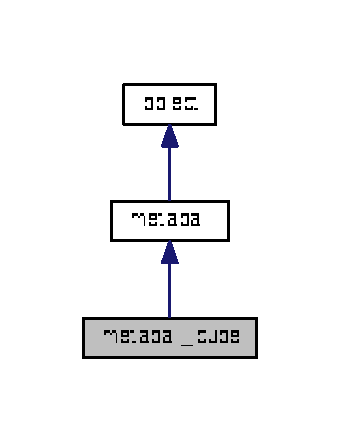
\includegraphics[width=163pt]{classmetaball__cube__inherit__graph}
\end{center}
\end{figure}


Collaboration diagram for metaball\+\_\+cube\+:\nopagebreak
\begin{figure}[H]
\begin{center}
\leavevmode
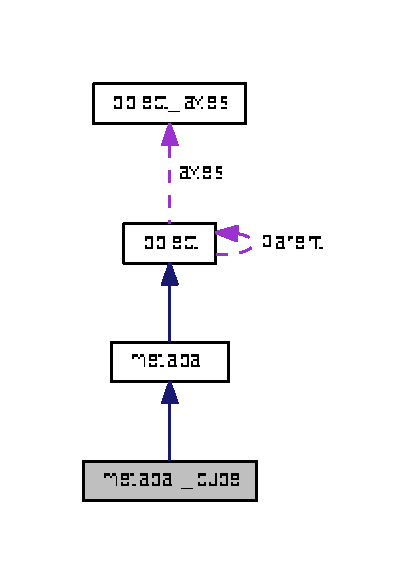
\includegraphics[width=196pt]{classmetaball__cube__coll__graph}
\end{center}
\end{figure}
\subsection*{Additional Inherited Members}


The documentation for this class was generated from the following file\+:\begin{DoxyCompactItemize}
\item 
include/metaball.\+h\end{DoxyCompactItemize}

\hypertarget{classmetaball__cylinder}{}\section{metaball\+\_\+cylinder Class Reference}
\label{classmetaball__cylinder}\index{metaball\+\_\+cylinder@{metaball\+\_\+cylinder}}


Inheritance diagram for metaball\+\_\+cylinder\+:\nopagebreak
\begin{figure}[H]
\begin{center}
\leavevmode
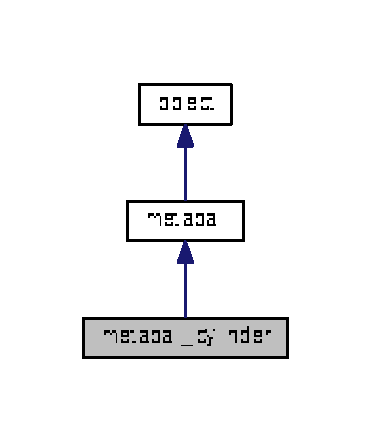
\includegraphics[width=178pt]{classmetaball__cylinder__inherit__graph}
\end{center}
\end{figure}


Collaboration diagram for metaball\+\_\+cylinder\+:\nopagebreak
\begin{figure}[H]
\begin{center}
\leavevmode
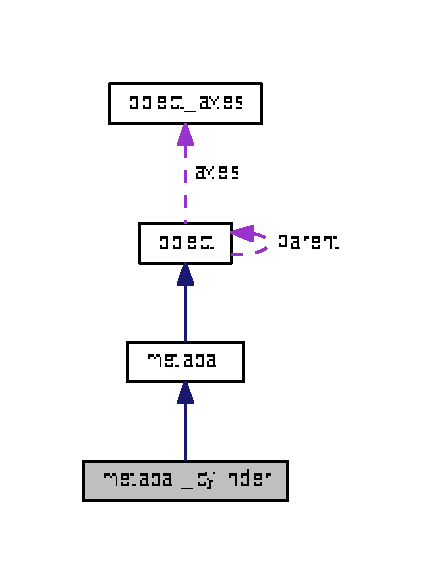
\includegraphics[width=203pt]{classmetaball__cylinder__coll__graph}
\end{center}
\end{figure}
\subsection*{Additional Inherited Members}


The documentation for this class was generated from the following file\+:\begin{DoxyCompactItemize}
\item 
include/metaball.\+h\end{DoxyCompactItemize}

\hypertarget{classmetaball__muscle}{}\section{metaball\+\_\+muscle Class Reference}
\label{classmetaball__muscle}\index{metaball\+\_\+muscle@{metaball\+\_\+muscle}}


Inheritance diagram for metaball\+\_\+muscle\+:\nopagebreak
\begin{figure}[H]
\begin{center}
\leavevmode
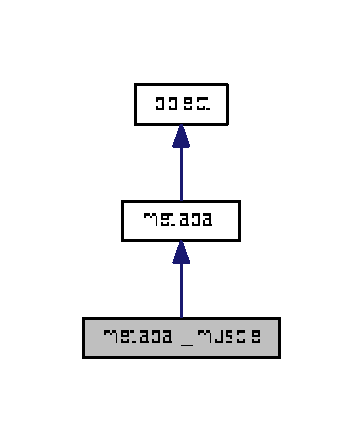
\includegraphics[width=174pt]{classmetaball__muscle__inherit__graph}
\end{center}
\end{figure}


Collaboration diagram for metaball\+\_\+muscle\+:\nopagebreak
\begin{figure}[H]
\begin{center}
\leavevmode
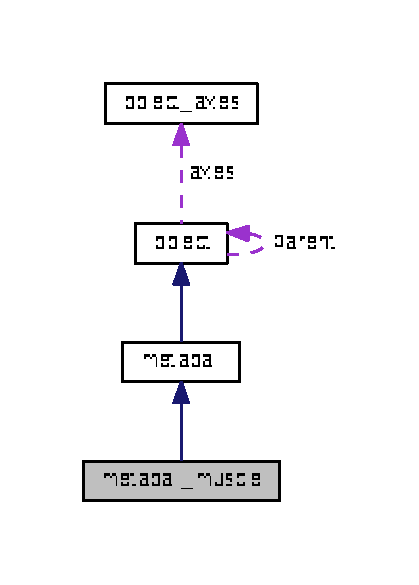
\includegraphics[width=201pt]{classmetaball__muscle__coll__graph}
\end{center}
\end{figure}
\subsection*{Additional Inherited Members}


The documentation for this class was generated from the following file\+:\begin{DoxyCompactItemize}
\item 
include/metaball.\+h\end{DoxyCompactItemize}

\hypertarget{classmetaball__rounded__cube}{}\section{metaball\+\_\+rounded\+\_\+cube Class Reference}
\label{classmetaball__rounded__cube}\index{metaball\+\_\+rounded\+\_\+cube@{metaball\+\_\+rounded\+\_\+cube}}


Inheritance diagram for metaball\+\_\+rounded\+\_\+cube\+:\nopagebreak
\begin{figure}[H]
\begin{center}
\leavevmode
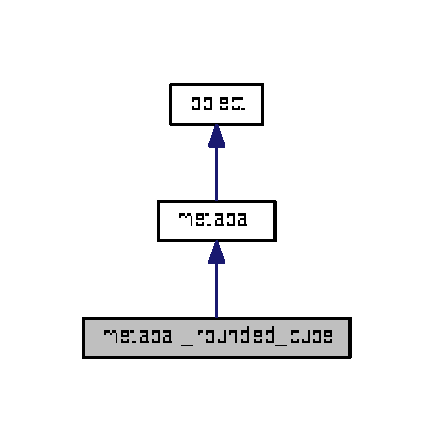
\includegraphics[width=208pt]{classmetaball__rounded__cube__inherit__graph}
\end{center}
\end{figure}


Collaboration diagram for metaball\+\_\+rounded\+\_\+cube\+:\nopagebreak
\begin{figure}[H]
\begin{center}
\leavevmode
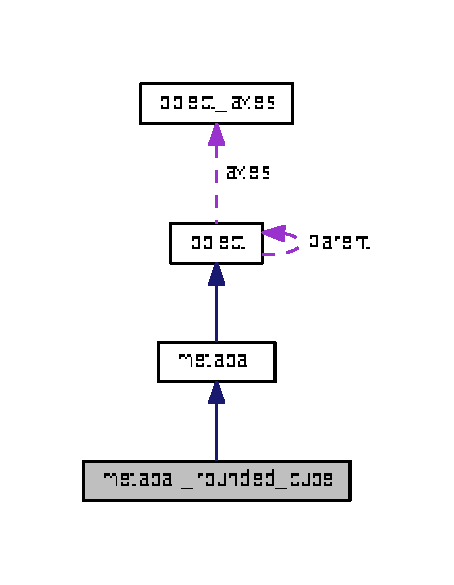
\includegraphics[width=218pt]{classmetaball__rounded__cube__coll__graph}
\end{center}
\end{figure}
\subsection*{Additional Inherited Members}


The documentation for this class was generated from the following file\+:\begin{DoxyCompactItemize}
\item 
include/metaball.\+h\end{DoxyCompactItemize}

\hypertarget{classmetaball__rounded__cylinder}{}\section{metaball\+\_\+rounded\+\_\+cylinder Class Reference}
\label{classmetaball__rounded__cylinder}\index{metaball\+\_\+rounded\+\_\+cylinder@{metaball\+\_\+rounded\+\_\+cylinder}}


Inheritance diagram for metaball\+\_\+rounded\+\_\+cylinder\+:\nopagebreak
\begin{figure}[H]
\begin{center}
\leavevmode
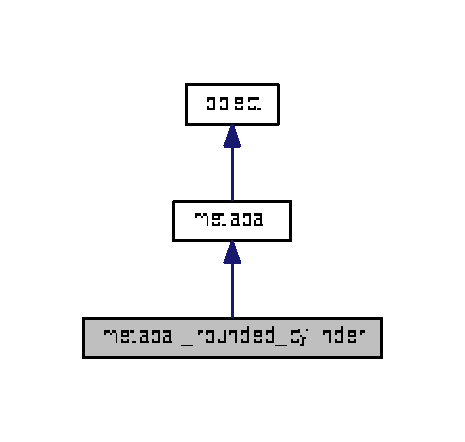
\includegraphics[width=223pt]{classmetaball__rounded__cylinder__inherit__graph}
\end{center}
\end{figure}


Collaboration diagram for metaball\+\_\+rounded\+\_\+cylinder\+:\nopagebreak
\begin{figure}[H]
\begin{center}
\leavevmode
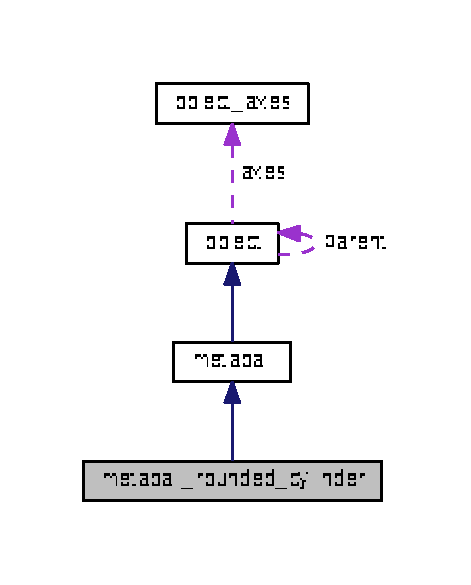
\includegraphics[width=226pt]{classmetaball__rounded__cylinder__coll__graph}
\end{center}
\end{figure}
\subsection*{Additional Inherited Members}


The documentation for this class was generated from the following file\+:\begin{DoxyCompactItemize}
\item 
include/metaball.\+h\end{DoxyCompactItemize}

\hypertarget{classmetaball__sphere}{}\section{metaball\+\_\+sphere Class Reference}
\label{classmetaball__sphere}\index{metaball\+\_\+sphere@{metaball\+\_\+sphere}}


Inheritance diagram for metaball\+\_\+sphere\+:\nopagebreak
\begin{figure}[H]
\begin{center}
\leavevmode
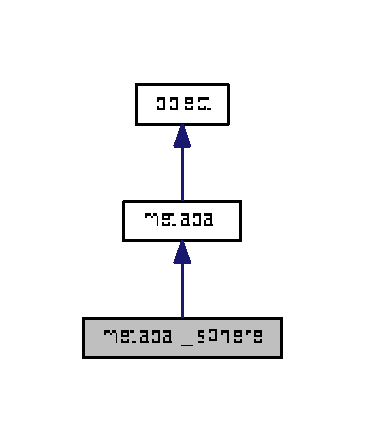
\includegraphics[width=175pt]{classmetaball__sphere__inherit__graph}
\end{center}
\end{figure}


Collaboration diagram for metaball\+\_\+sphere\+:\nopagebreak
\begin{figure}[H]
\begin{center}
\leavevmode
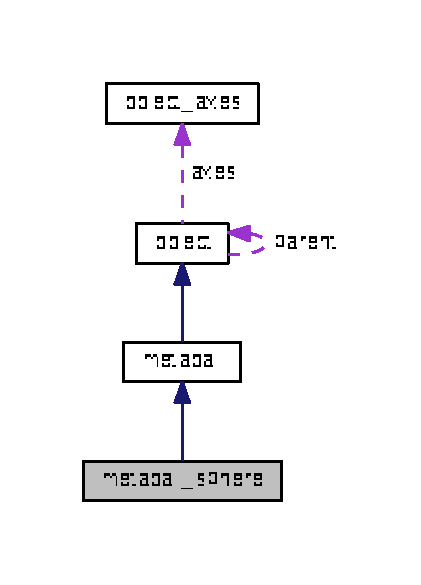
\includegraphics[width=202pt]{classmetaball__sphere__coll__graph}
\end{center}
\end{figure}
\subsection*{Additional Inherited Members}


The documentation for this class was generated from the following file\+:\begin{DoxyCompactItemize}
\item 
include/metaball.\+h\end{DoxyCompactItemize}

\hypertarget{structmg2__frame}{}\section{mg2\+\_\+frame Struct Reference}
\label{structmg2__frame}\index{mg2\+\_\+frame@{mg2\+\_\+frame}}
\subsection*{Public Attributes}
\begin{DoxyCompactItemize}
\item 
\mbox{\Hypertarget{structmg2__frame_a2762c5b7d2b5a6fe182235c69e510d21}\label{structmg2__frame_a2762c5b7d2b5a6fe182235c69e510d21}} 
char {\bfseries is\+\_\+keyframe}
\item 
\mbox{\Hypertarget{structmg2__frame_ad0301a9960f8908da384479f846924cf}\label{structmg2__frame_ad0301a9960f8908da384479f846924cf}} 
float {\bfseries rotate} \mbox{[}16\mbox{]}
\item 
\mbox{\Hypertarget{structmg2__frame_a3709feba21e54155ca961f0b335c163d}\label{structmg2__frame_a3709feba21e54155ca961f0b335c163d}} 
float {\bfseries translate} \mbox{[}3\mbox{]}
\item 
\mbox{\Hypertarget{structmg2__frame_a16a198b1823d5d3ebb46b71cacd451a5}\label{structmg2__frame_a16a198b1823d5d3ebb46b71cacd451a5}} 
float {\bfseries scale} \mbox{[}3\mbox{]}
\end{DoxyCompactItemize}


The documentation for this struct was generated from the following file\+:\begin{DoxyCompactItemize}
\item 
include/mg2.\+h\end{DoxyCompactItemize}

\hypertarget{structmg2__material}{}\section{mg2\+\_\+material Struct Reference}
\label{structmg2__material}\index{mg2\+\_\+material@{mg2\+\_\+material}}
\subsection*{Public Attributes}
\begin{DoxyCompactItemize}
\item 
\mbox{\Hypertarget{structmg2__material_a3a3c5275b02d07dc34aec02fc9f9d5ca}\label{structmg2__material_a3a3c5275b02d07dc34aec02fc9f9d5ca}} 
gulong {\bfseries ref\+\_\+count}
\item 
\mbox{\Hypertarget{structmg2__material_a77c1d7656583d004e9fd67fc291c8b0c}\label{structmg2__material_a77c1d7656583d004e9fd67fc291c8b0c}} 
float {\bfseries ambient} \mbox{[}4\mbox{]}
\item 
\mbox{\Hypertarget{structmg2__material_a627b9e332c960ed7845881420a5d5811}\label{structmg2__material_a627b9e332c960ed7845881420a5d5811}} 
float {\bfseries diffuse} \mbox{[}4\mbox{]}
\item 
\mbox{\Hypertarget{structmg2__material_a79601f83d3341cea3608c08bf5db4aa8}\label{structmg2__material_a79601f83d3341cea3608c08bf5db4aa8}} 
float {\bfseries specular} \mbox{[}4\mbox{]}
\item 
\mbox{\Hypertarget{structmg2__material_a10466fcd31fc382de388a2d4b0046603}\label{structmg2__material_a10466fcd31fc382de388a2d4b0046603}} 
float {\bfseries shininess}
\item 
\mbox{\Hypertarget{structmg2__material_a43c300b9ed72d5c7d0417abd962aa90c}\label{structmg2__material_a43c300b9ed72d5c7d0417abd962aa90c}} 
float {\bfseries emission} \mbox{[}4\mbox{]}
\item 
\mbox{\Hypertarget{structmg2__material_aba5ac031bce0a3ae0e45c4d892e61af9}\label{structmg2__material_aba5ac031bce0a3ae0e45c4d892e61af9}} 
G\+Luint {\bfseries textureid}
\item 
\mbox{\Hypertarget{structmg2__material_a594b57d523ae2020f7fa322cf4b7c6dc}\label{structmg2__material_a594b57d523ae2020f7fa322cf4b7c6dc}} 
guint {\bfseries material\+\_\+list}
\end{DoxyCompactItemize}


The documentation for this struct was generated from the following file\+:\begin{DoxyCompactItemize}
\item 
include/mg2.\+h\end{DoxyCompactItemize}

\hypertarget{structmg2__vertex}{}\section{mg2\+\_\+vertex Struct Reference}
\label{structmg2__vertex}\index{mg2\+\_\+vertex@{mg2\+\_\+vertex}}
\subsection*{Public Attributes}
\begin{DoxyCompactItemize}
\item 
\mbox{\Hypertarget{structmg2__vertex_a76756f1c82bf50b7e91821429df4ffef}\label{structmg2__vertex_a76756f1c82bf50b7e91821429df4ffef}} 
gfloat {\bfseries p} \mbox{[}3\mbox{]}
\end{DoxyCompactItemize}


The documentation for this struct was generated from the following file\+:\begin{DoxyCompactItemize}
\item 
include/mg2.\+h\end{DoxyCompactItemize}

\hypertarget{classnormal}{}\section{normal Class Reference}
\label{classnormal}\index{normal@{normal}}


The documentation for this class was generated from the following file\+:\begin{DoxyCompactItemize}
\item 
include/normal.\+h\end{DoxyCompactItemize}

\hypertarget{classnurbs}{}\section{nurbs Class Reference}
\label{classnurbs}\index{nurbs@{nurbs}}


Inheritance diagram for nurbs\+:\nopagebreak
\begin{figure}[H]
\begin{center}
\leavevmode
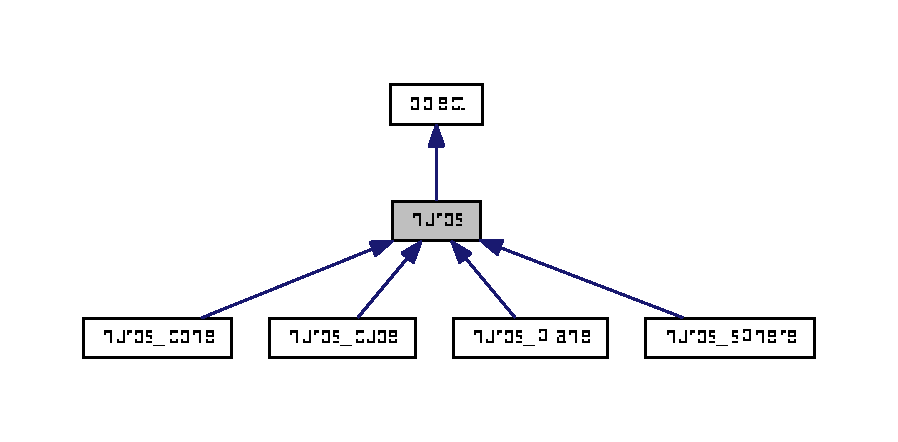
\includegraphics[width=350pt]{classnurbs__inherit__graph}
\end{center}
\end{figure}


Collaboration diagram for nurbs\+:\nopagebreak
\begin{figure}[H]
\begin{center}
\leavevmode
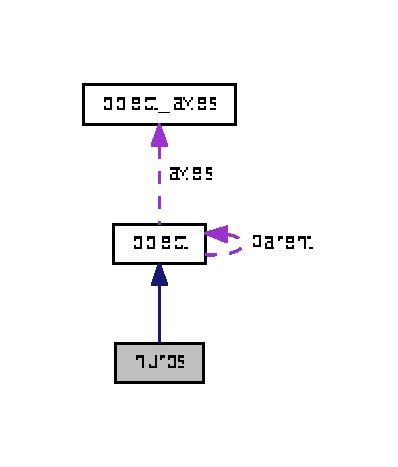
\includegraphics[width=191pt]{classnurbs__coll__graph}
\end{center}
\end{figure}
\subsection*{Additional Inherited Members}


The documentation for this class was generated from the following file\+:\begin{DoxyCompactItemize}
\item 
include/nurbs.\+h\end{DoxyCompactItemize}

\hypertarget{classnurbs__cone}{}\section{nurbs\+\_\+cone Class Reference}
\label{classnurbs__cone}\index{nurbs\+\_\+cone@{nurbs\+\_\+cone}}


Inheritance diagram for nurbs\+\_\+cone\+:\nopagebreak
\begin{figure}[H]
\begin{center}
\leavevmode
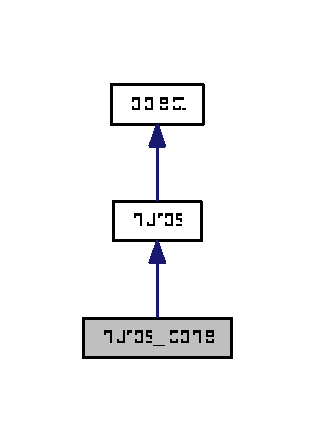
\includegraphics[width=151pt]{classnurbs__cone__inherit__graph}
\end{center}
\end{figure}


Collaboration diagram for nurbs\+\_\+cone\+:\nopagebreak
\begin{figure}[H]
\begin{center}
\leavevmode
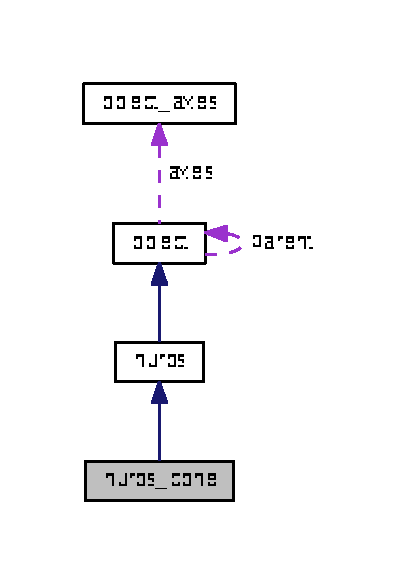
\includegraphics[width=191pt]{classnurbs__cone__coll__graph}
\end{center}
\end{figure}
\subsection*{Additional Inherited Members}


The documentation for this class was generated from the following file\+:\begin{DoxyCompactItemize}
\item 
include/nurbs.\+h\end{DoxyCompactItemize}

\hypertarget{classnurbs__cube}{}\section{nurbs\+\_\+cube Class Reference}
\label{classnurbs__cube}\index{nurbs\+\_\+cube@{nurbs\+\_\+cube}}


Inheritance diagram for nurbs\+\_\+cube\+:\nopagebreak
\begin{figure}[H]
\begin{center}
\leavevmode
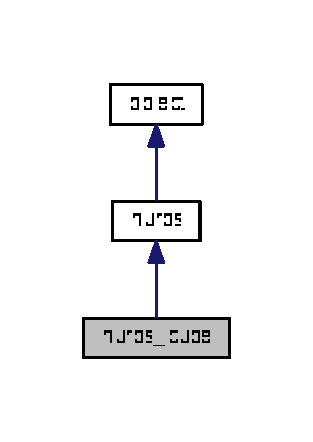
\includegraphics[width=150pt]{classnurbs__cube__inherit__graph}
\end{center}
\end{figure}


Collaboration diagram for nurbs\+\_\+cube\+:\nopagebreak
\begin{figure}[H]
\begin{center}
\leavevmode
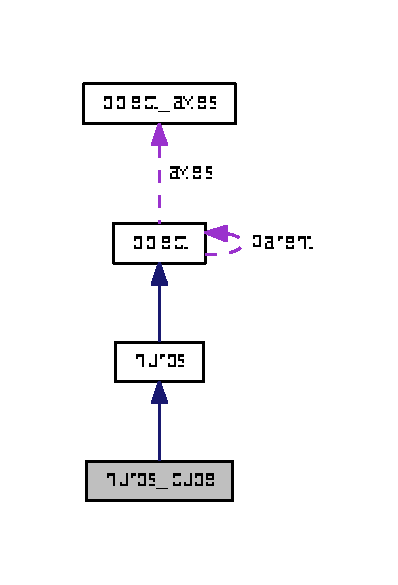
\includegraphics[width=191pt]{classnurbs__cube__coll__graph}
\end{center}
\end{figure}
\subsection*{Additional Inherited Members}


The documentation for this class was generated from the following file\+:\begin{DoxyCompactItemize}
\item 
include/nurbs.\+h\end{DoxyCompactItemize}

\hypertarget{classnurbs__plane}{}\section{nurbs\+\_\+plane Class Reference}
\label{classnurbs__plane}\index{nurbs\+\_\+plane@{nurbs\+\_\+plane}}


Inheritance diagram for nurbs\+\_\+plane\+:\nopagebreak
\begin{figure}[H]
\begin{center}
\leavevmode
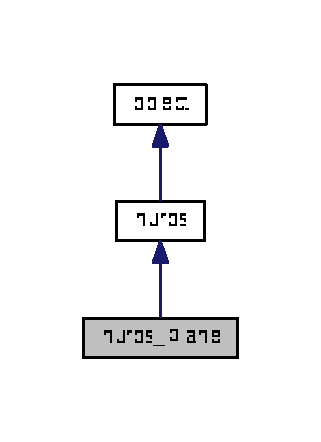
\includegraphics[width=154pt]{classnurbs__plane__inherit__graph}
\end{center}
\end{figure}


Collaboration diagram for nurbs\+\_\+plane\+:\nopagebreak
\begin{figure}[H]
\begin{center}
\leavevmode
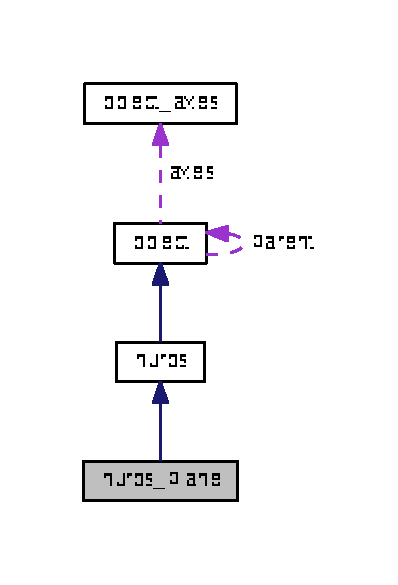
\includegraphics[width=191pt]{classnurbs__plane__coll__graph}
\end{center}
\end{figure}
\subsection*{Additional Inherited Members}


The documentation for this class was generated from the following file\+:\begin{DoxyCompactItemize}
\item 
include/nurbs.\+h\end{DoxyCompactItemize}

\hypertarget{classnurbs__sphere}{}\section{nurbs\+\_\+sphere Class Reference}
\label{classnurbs__sphere}\index{nurbs\+\_\+sphere@{nurbs\+\_\+sphere}}


Inheritance diagram for nurbs\+\_\+sphere\+:\nopagebreak
\begin{figure}[H]
\begin{center}
\leavevmode
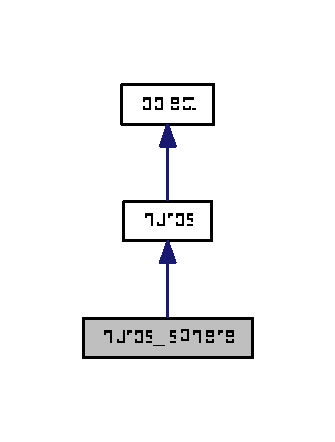
\includegraphics[width=161pt]{classnurbs__sphere__inherit__graph}
\end{center}
\end{figure}


Collaboration diagram for nurbs\+\_\+sphere\+:\nopagebreak
\begin{figure}[H]
\begin{center}
\leavevmode
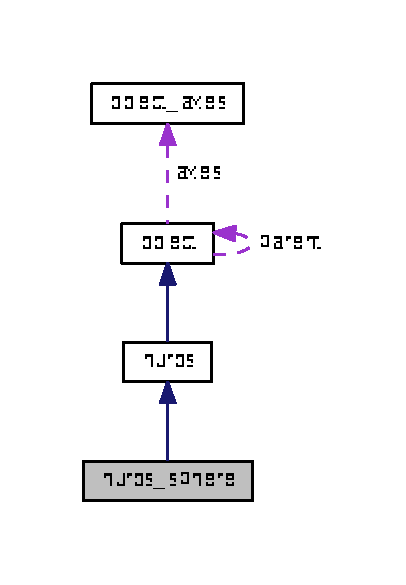
\includegraphics[width=195pt]{classnurbs__sphere__coll__graph}
\end{center}
\end{figure}
\subsection*{Additional Inherited Members}


The documentation for this class was generated from the following file\+:\begin{DoxyCompactItemize}
\item 
include/nurbs.\+h\end{DoxyCompactItemize}

\hypertarget{classobject}{}\section{object Class Reference}
\label{classobject}\index{object@{object}}


Inheritance diagram for object\+:
\nopagebreak
\begin{figure}[H]
\begin{center}
\leavevmode
\includegraphics[height=550pt]{classobject__inherit__graph}
\end{center}
\end{figure}


Collaboration diagram for object\+:\nopagebreak
\begin{figure}[H]
\begin{center}
\leavevmode
\includegraphics[width=191pt]{classobject__coll__graph}
\end{center}
\end{figure}
\subsection*{Public Member Functions}
\begin{DoxyCompactItemize}
\item 
\mbox{\Hypertarget{classobject_a049bf210513dcad8befc446b21bbe04e}\label{classobject_a049bf210513dcad8befc446b21bbe04e}} 
void {\bfseries Set\+Location} (double loc\+\_\+X, double loc\+\_\+Y, double loc\+\_\+Z)
\item 
\mbox{\Hypertarget{classobject_a76a69357efa11fcc74550e98ada78be4}\label{classobject_a76a69357efa11fcc74550e98ada78be4}} 
void {\bfseries Set\+Rotation} (double rot\+\_\+X, double rot\+\_\+Y, double rot\+\_\+Z)
\item 
\mbox{\Hypertarget{classobject_a3851ac40d2ece1b7773b473c6b0cbeb9}\label{classobject_a3851ac40d2ece1b7773b473c6b0cbeb9}} 
void {\bfseries Set\+Scale} (double sca\+\_\+X, double sca\+\_\+Y, double sca\+\_\+Z)
\item 
\mbox{\Hypertarget{classobject_a08fc87e448cd19e7b39063909b79335b}\label{classobject_a08fc87e448cd19e7b39063909b79335b}} 
int $\ast$ {\bfseries Get\+Location} ()
\item 
\mbox{\Hypertarget{classobject_a963b5696150b7950c5103f8f5da316fc}\label{classobject_a963b5696150b7950c5103f8f5da316fc}} 
int $\ast$ {\bfseries Get\+Rotation} ()
\item 
\mbox{\Hypertarget{classobject_a6b698fe06532b0311f9fac0d6c377076}\label{classobject_a6b698fe06532b0311f9fac0d6c377076}} 
int $\ast$ {\bfseries Get\+Scale} ()
\item 
\mbox{\Hypertarget{classobject_ac9e1f82f9673d009e293d2866bb12185}\label{classobject_ac9e1f82f9673d009e293d2866bb12185}} 
int {\bfseries Get\+Num\+Vertices} ()
\item 
\mbox{\Hypertarget{classobject_a55064bb9cec74c348aa9c6b63828c413}\label{classobject_a55064bb9cec74c348aa9c6b63828c413}} 
int {\bfseries Get\+Num\+Faces} ()
\item 
\mbox{\Hypertarget{classobject_acaf5c6b0f64d5044a487c6a89832b110}\label{classobject_acaf5c6b0f64d5044a487c6a89832b110}} 
void {\bfseries Set\+Num\+Vertices} (int num\+\_\+vertices)
\item 
\mbox{\Hypertarget{classobject_a85014bdbe0bfa2558d806d7faa7219e6}\label{classobject_a85014bdbe0bfa2558d806d7faa7219e6}} 
void {\bfseries Set\+Num\+Faces} (int num\+\_\+faces)
\item 
\mbox{\Hypertarget{classobject_a4263222470132b9ff0bd23e981f6d15c}\label{classobject_a4263222470132b9ff0bd23e981f6d15c}} 
void {\bfseries Add\+Child} (\hyperlink{classobject}{object} $\ast$child)
\item 
\mbox{\Hypertarget{classobject_a19ce6355c2d3c1bf315190e6ac45c382}\label{classobject_a19ce6355c2d3c1bf315190e6ac45c382}} 
void {\bfseries Remove\+Child} (\hyperlink{classobject}{object} $\ast$child)
\item 
\mbox{\Hypertarget{classobject_a2c381e2defde6ee24acca434e6ee9fd0}\label{classobject_a2c381e2defde6ee24acca434e6ee9fd0}} 
void {\bfseries Enable\+Axes} (bool show\+\_\+axes)
\item 
\mbox{\Hypertarget{classobject_a287c47ea62fed1e3ece7ff6ac0398ea1}\label{classobject_a287c47ea62fed1e3ece7ff6ac0398ea1}} 
void {\bfseries Enable\+Origin} (bool show\+\_\+origin)
\item 
\mbox{\Hypertarget{classobject_a732616252ee8004c41b496905f1f8604}\label{classobject_a732616252ee8004c41b496905f1f8604}} 
void {\bfseries Add\+Frame} (void)
\item 
\mbox{\Hypertarget{classobject_a39c3249be7b37b58c319b4f3c6311eda}\label{classobject_a39c3249be7b37b58c319b4f3c6311eda}} 
void {\bfseries Remove\+Frame} (\hyperlink{classframe}{frame} $\ast$\hyperlink{classframe}{frame})
\end{DoxyCompactItemize}
\subsection*{Public Attributes}
\begin{DoxyCompactItemize}
\item 
\mbox{\Hypertarget{classobject_af115c45426fbea680786bc80825b36c7}\label{classobject_af115c45426fbea680786bc80825b36c7}} 
int {\bfseries location} \mbox{[}3\mbox{]}
\item 
\mbox{\Hypertarget{classobject_a4ed36f5119af885c3cca2a34a246a99d}\label{classobject_a4ed36f5119af885c3cca2a34a246a99d}} 
int {\bfseries rotation} \mbox{[}3\mbox{]}
\item 
\mbox{\Hypertarget{classobject_a138d43dace4c2628aa85fa3bf4c9545f}\label{classobject_a138d43dace4c2628aa85fa3bf4c9545f}} 
int {\bfseries scale} \mbox{[}3\mbox{]}
\item 
\mbox{\Hypertarget{classobject_a1cc7d0fccb248da1c6e16ea36bbbbfe2}\label{classobject_a1cc7d0fccb248da1c6e16ea36bbbbfe2}} 
string {\bfseries name}
\item 
\mbox{\Hypertarget{classobject_a251f1cd9e5cff874f7bd2ac2d1adb838}\label{classobject_a251f1cd9e5cff874f7bd2ac2d1adb838}} 
float {\bfseries selected\+\_\+color} \mbox{[}3\mbox{]}
\item 
\mbox{\Hypertarget{classobject_aff12337bfe21bab93b31bf19e0a8f441}\label{classobject_aff12337bfe21bab93b31bf19e0a8f441}} 
float {\bfseries unselected\+\_\+color} \mbox{[}3\mbox{]}
\item 
\mbox{\Hypertarget{classobject_a10204a3a1993a47bcea7bfd2a3624f23}\label{classobject_a10204a3a1993a47bcea7bfd2a3624f23}} 
int {\bfseries num\+\_\+vertices}
\item 
\mbox{\Hypertarget{classobject_ac03c0ba2b5c8af232a007d53d4d4403e}\label{classobject_ac03c0ba2b5c8af232a007d53d4d4403e}} 
int {\bfseries num\+\_\+faces}
\item 
\mbox{\Hypertarget{classobject_a087c94dd665b5ba400f6b8a5173a8712}\label{classobject_a087c94dd665b5ba400f6b8a5173a8712}} 
int {\bfseries num\+\_\+frames}
\item 
\mbox{\Hypertarget{classobject_aa46ff2afb44d3db473279693e625974a}\label{classobject_aa46ff2afb44d3db473279693e625974a}} 
bool {\bfseries is\+\_\+parent\+\_\+only}
\item 
\mbox{\Hypertarget{classobject_ae0050cfb8a9d4270f90e2becfc4d5057}\label{classobject_ae0050cfb8a9d4270f90e2becfc4d5057}} 
\hyperlink{classobject}{object} $\ast$ {\bfseries parent}
\item 
\mbox{\Hypertarget{classobject_a1a313581b8358481d9c42bff8b7f6c42}\label{classobject_a1a313581b8358481d9c42bff8b7f6c42}} 
list$<$ \hyperlink{classobject}{object} $>$ {\bfseries children}
\item 
\mbox{\Hypertarget{classobject_a7278bfffc4704696520683bfb395da44}\label{classobject_a7278bfffc4704696520683bfb395da44}} 
list$<$ \hyperlink{classvertex}{vertex} $>$ {\bfseries vertices}
\item 
\mbox{\Hypertarget{classobject_abc60cb2c258fcbda52a3b837cf9e3abf}\label{classobject_abc60cb2c258fcbda52a3b837cf9e3abf}} 
list$<$ \hyperlink{classedge}{edge} $>$ {\bfseries edges}
\item 
\mbox{\Hypertarget{classobject_a957ee3e1d2491444a7879ed81c10eca2}\label{classobject_a957ee3e1d2491444a7879ed81c10eca2}} 
list$<$ \hyperlink{classface}{face} $>$ {\bfseries faces}
\item 
\mbox{\Hypertarget{classobject_a5ee08f3f3b0ec7b3a1406226ac4a472b}\label{classobject_a5ee08f3f3b0ec7b3a1406226ac4a472b}} 
list$<$ \hyperlink{classnormal}{normal} $>$ {\bfseries normals}
\item 
\mbox{\Hypertarget{classobject_a1c5324d2586aca3c0fd280ac075eb306}\label{classobject_a1c5324d2586aca3c0fd280ac075eb306}} 
float {\bfseries origin} \mbox{[}3\mbox{]}
\item 
\mbox{\Hypertarget{classobject_a37f599665f13088b41ef2638d6ba164f}\label{classobject_a37f599665f13088b41ef2638d6ba164f}} 
bool {\bfseries show\+\_\+axes}
\item 
\mbox{\Hypertarget{classobject_a54652d62b451828b36c87194986b5943}\label{classobject_a54652d62b451828b36c87194986b5943}} 
\hyperlink{structobject__axes}{object\+\_\+axes} {\bfseries axes}
\item 
\mbox{\Hypertarget{classobject_a18d91cc7a213dd0578e44b2984e5ec90}\label{classobject_a18d91cc7a213dd0578e44b2984e5ec90}} 
bool {\bfseries show\+\_\+origin}
\item 
\mbox{\Hypertarget{classobject_a19883eb1b024497eb465b3708e813f60}\label{classobject_a19883eb1b024497eb465b3708e813f60}} 
float {\bfseries compensation} \mbox{[}16\mbox{]}
\item 
\mbox{\Hypertarget{classobject_a21d0a6ebc2f0040aed7e3596e5b2f72e}\label{classobject_a21d0a6ebc2f0040aed7e3596e5b2f72e}} 
float {\bfseries rot\+\_\+origin} \mbox{[}16\mbox{]}
\item 
\mbox{\Hypertarget{classobject_ae50c6097bb51f8105dec67e5164d642e}\label{classobject_ae50c6097bb51f8105dec67e5164d642e}} 
list$<$ \hyperlink{classframe}{frame} $>$ {\bfseries frames}
\end{DoxyCompactItemize}


The documentation for this class was generated from the following files\+:\begin{DoxyCompactItemize}
\item 
include/object.\+h\item 
src/object.\+cpp\end{DoxyCompactItemize}

\hypertarget{structobject__axes}{}\section{object\+\_\+axes Struct Reference}
\label{structobject__axes}\index{object\+\_\+axes@{object\+\_\+axes}}
\subsection*{Public Attributes}
\begin{DoxyCompactItemize}
\item 
\mbox{\Hypertarget{structobject__axes_a0d04d612437076c541cf3bc70434b2ce}\label{structobject__axes_a0d04d612437076c541cf3bc70434b2ce}} 
float {\bfseries axes} \mbox{[}3\mbox{]}
\end{DoxyCompactItemize}


The documentation for this struct was generated from the following file\+:\begin{DoxyCompactItemize}
\item 
include/geometry.\+h\end{DoxyCompactItemize}

\hypertarget{classpanoramic__camera}{}\section{panoramic\+\_\+camera Class Reference}
\label{classpanoramic__camera}\index{panoramic\+\_\+camera@{panoramic\+\_\+camera}}


Inheritance diagram for panoramic\+\_\+camera\+:\nopagebreak
\begin{figure}[H]
\begin{center}
\leavevmode
\includegraphics[width=187pt]{classpanoramic__camera__inherit__graph}
\end{center}
\end{figure}


Collaboration diagram for panoramic\+\_\+camera\+:\nopagebreak
\begin{figure}[H]
\begin{center}
\leavevmode
\includegraphics[width=208pt]{classpanoramic__camera__coll__graph}
\end{center}
\end{figure}
\subsection*{Additional Inherited Members}


The documentation for this class was generated from the following file\+:\begin{DoxyCompactItemize}
\item 
include/camera.\+h\end{DoxyCompactItemize}

\hypertarget{classplane}{}\section{plane Class Reference}
\label{classplane}\index{plane@{plane}}


Inheritance diagram for plane\+:\nopagebreak
\begin{figure}[H]
\begin{center}
\leavevmode
\includegraphics[width=136pt]{classplane__inherit__graph}
\end{center}
\end{figure}


Collaboration diagram for plane\+:\nopagebreak
\begin{figure}[H]
\begin{center}
\leavevmode
\includegraphics[width=191pt]{classplane__coll__graph}
\end{center}
\end{figure}
\subsection*{Public Member Functions}
\begin{DoxyCompactItemize}
\item 
\mbox{\Hypertarget{classplane_acc9f6a598cf1ea430521388697825229}\label{classplane_acc9f6a598cf1ea430521388697825229}} 
void {\bfseries make\+\_\+plane} (int horizontal\+\_\+subdiv, int vertical\+\_\+subdiv, int conic\+\_\+subdiv, int spherical\+\_\+long\+\_\+subdiv, int spherical\+\_\+lat\+\_\+subdiv, int x\+\_\+rotation, int torus\+\_\+angle, int top\+\_\+radius, int bot\+\_\+radius, int radius, int spherical\+\_\+radius, int conic\+\_\+angle, int height, int rot\+\_\+subdiv)
\end{DoxyCompactItemize}


The documentation for this class was generated from the following files\+:\begin{DoxyCompactItemize}
\item 
include/primitive.\+h\item 
src/primitive.\+cpp\end{DoxyCompactItemize}

\hypertarget{structpos__color__vertex}{}\section{pos\+\_\+color\+\_\+vertex Struct Reference}
\label{structpos__color__vertex}\index{pos\+\_\+color\+\_\+vertex@{pos\+\_\+color\+\_\+vertex}}
\subsection*{Public Attributes}
\begin{DoxyCompactItemize}
\item 
\mbox{\Hypertarget{structpos__color__vertex_a3fe1392c96e92389560c8f1b07bf56fe}\label{structpos__color__vertex_a3fe1392c96e92389560c8f1b07bf56fe}} 
float {\bfseries pos} \mbox{[}3\mbox{]}
\item 
\mbox{\Hypertarget{structpos__color__vertex_af66a8b148a74fdaeea34da46baaa1009}\label{structpos__color__vertex_af66a8b148a74fdaeea34da46baaa1009}} 
float {\bfseries color} \mbox{[}3\mbox{]}
\end{DoxyCompactItemize}


The documentation for this struct was generated from the following file\+:\begin{DoxyCompactItemize}
\item 
src/object.\+cpp\end{DoxyCompactItemize}

\hypertarget{classpreferences}{}\section{preferences Class Reference}
\label{classpreferences}\index{preferences@{preferences}}
\subsection*{Public Member Functions}
\begin{DoxyCompactItemize}
\item 
\mbox{\Hypertarget{classpreferences_a35f7b6a82f35749a7d0d4a42073cdcf4}\label{classpreferences_a35f7b6a82f35749a7d0d4a42073cdcf4}} 
void {\bfseries default\+\_\+preferences} (void)
\item 
\mbox{\Hypertarget{classpreferences_a679949faa2166d83d002d234f6394b9f}\label{classpreferences_a679949faa2166d83d002d234f6394b9f}} 
void {\bfseries load\+\_\+preferences} (string filename)
\item 
\mbox{\Hypertarget{classpreferences_ab02600d9ef05e3cfb6263e3fe4dce85c}\label{classpreferences_ab02600d9ef05e3cfb6263e3fe4dce85c}} 
void {\bfseries save\+\_\+preferences} (string filename)
\item 
\mbox{\Hypertarget{classpreferences_a6fbbdf1ac3a3b0b154d693c328b0f025}\label{classpreferences_a6fbbdf1ac3a3b0b154d693c328b0f025}} 
void {\bfseries set\+\_\+interface\+\_\+type} (int interface\+\_\+type)
\item 
\mbox{\Hypertarget{classpreferences_a6dfb48f950f7ca18b5aadc0c45f5872f}\label{classpreferences_a6dfb48f950f7ca18b5aadc0c45f5872f}} 
void {\bfseries set\+\_\+grid\+\_\+resolution} (int grid\+\_\+resolution)
\item 
\mbox{\Hypertarget{classpreferences_ab525e5b6273a19190fec0c2bd6c0605a}\label{classpreferences_ab525e5b6273a19190fec0c2bd6c0605a}} 
void {\bfseries set\+\_\+draw\+\_\+ground\+\_\+plane} (bool draw\+\_\+ground\+\_\+plane)
\item 
\mbox{\Hypertarget{classpreferences_afbdc7487245f6e1c2f26c3ef7ba986fa}\label{classpreferences_afbdc7487245f6e1c2f26c3ef7ba986fa}} 
void {\bfseries set\+\_\+draw\+\_\+axes} (bool draw\+\_\+axes)
\item 
\mbox{\Hypertarget{classpreferences_a0d2136cfbbad55bfaf64eae9549bd68e}\label{classpreferences_a0d2136cfbbad55bfaf64eae9549bd68e}} 
int {\bfseries get\+\_\+interface\+\_\+type} ()
\item 
\mbox{\Hypertarget{classpreferences_a9cd938457a3d4387017fcbd6f6a489b1}\label{classpreferences_a9cd938457a3d4387017fcbd6f6a489b1}} 
int {\bfseries get\+\_\+grid\+\_\+resolution} ()
\item 
\mbox{\Hypertarget{classpreferences_a790b34241f358007907fa3fda6978add}\label{classpreferences_a790b34241f358007907fa3fda6978add}} 
int {\bfseries get\+\_\+draw\+\_\+ground\+\_\+plane} ()
\item 
\mbox{\Hypertarget{classpreferences_ad1eec1245431960040efa6c31cc7c57b}\label{classpreferences_ad1eec1245431960040efa6c31cc7c57b}} 
bool {\bfseries get\+\_\+draw\+\_\+axes} ()
\end{DoxyCompactItemize}
\subsection*{Protected Attributes}
\begin{DoxyCompactItemize}
\item 
\mbox{\Hypertarget{classpreferences_af1b38ff175740032ff2aefe04b9b8cae}\label{classpreferences_af1b38ff175740032ff2aefe04b9b8cae}} 
int {\bfseries interface\+\_\+type} = 1
\item 
\mbox{\Hypertarget{classpreferences_ad80ddea45159b683bfe941857d05b78b}\label{classpreferences_ad80ddea45159b683bfe941857d05b78b}} 
int {\bfseries grid\+\_\+resolution} = 32
\item 
\mbox{\Hypertarget{classpreferences_a03312cf0d332c39edfdbe73430029634}\label{classpreferences_a03312cf0d332c39edfdbe73430029634}} 
bool {\bfseries draw\+\_\+axes} = T\+R\+UE
\item 
\mbox{\Hypertarget{classpreferences_a79576b34baf1fd09c5e9923e668e2c59}\label{classpreferences_a79576b34baf1fd09c5e9923e668e2c59}} 
bool {\bfseries draw\+\_\+ground\+\_\+plane} = F\+A\+L\+SE
\item 
\mbox{\Hypertarget{classpreferences_abc0a4ea42c94f872320038818947dbaa}\label{classpreferences_abc0a4ea42c94f872320038818947dbaa}} 
float {\bfseries Background\+\_\+\+Color} \mbox{[}3\mbox{]} = \{ 0.\+6, 0.\+6, 0.\+6 \}
\item 
\mbox{\Hypertarget{classpreferences_ad9910fda8495cf8308ee5cab48a7621d}\label{classpreferences_ad9910fda8495cf8308ee5cab48a7621d}} 
float {\bfseries Grid\+\_\+\+Color} \mbox{[}3\mbox{]} = \{ 0.\+7, 0.\+7, 0.\+7 \}
\item 
\mbox{\Hypertarget{classpreferences_a467b9249314615ffddf9443671c92fae}\label{classpreferences_a467b9249314615ffddf9443671c92fae}} 
float {\bfseries Highlight\+\_\+\+Color} \mbox{[}3\mbox{]} = \{ 1.\+0, 1.\+0, 1.\+0 \}
\item 
\mbox{\Hypertarget{classpreferences_a1f7ffb821d1d4713ffb4a76d1e3cb322}\label{classpreferences_a1f7ffb821d1d4713ffb4a76d1e3cb322}} 
float {\bfseries Pe\+Sel\+\_\+\+Color} \mbox{[}3\mbox{]} = \{ 1.\+0, 1.\+0, 1.\+0 \}
\item 
\mbox{\Hypertarget{classpreferences_abbb572146585238498f257a6b2428d0d}\label{classpreferences_abbb572146585238498f257a6b2428d0d}} 
float {\bfseries Selected\+\_\+\+Color} \mbox{[}3\mbox{]} = \{ 1.\+0, 1.\+0, 1.\+0 \}
\item 
\mbox{\Hypertarget{classpreferences_a80c1a321a2bc72a2cceca7187b206b9d}\label{classpreferences_a80c1a321a2bc72a2cceca7187b206b9d}} 
float {\bfseries Unselected\+\_\+\+Color} \mbox{[}3\mbox{]} = \{ 1.\+0, 1.\+0, 1.\+0 \}
\item 
\mbox{\Hypertarget{classpreferences_aef308c504780b24ad1b13b7f8f2a6480}\label{classpreferences_aef308c504780b24ad1b13b7f8f2a6480}} 
float {\bfseries Light\+\_\+\+Color} \mbox{[}3\mbox{]} = \{ 1.\+0, 1.\+0, 1.\+0 \}
\item 
\mbox{\Hypertarget{classpreferences_af9d020bef7c3d63de45b02cde80a8087}\label{classpreferences_af9d020bef7c3d63de45b02cde80a8087}} 
float {\bfseries Camera\+\_\+\+Color} \mbox{[}3\mbox{]} = \{ 1.\+0, 1.\+0, 1.\+0 \}
\end{DoxyCompactItemize}


The documentation for this class was generated from the following files\+:\begin{DoxyCompactItemize}
\item 
include/preferences.\+h\item 
src/preferences.\+cpp\end{DoxyCompactItemize}

\hypertarget{structpressrelease}{}\section{pressrelease Struct Reference}
\label{structpressrelease}\index{pressrelease@{pressrelease}}
\subsection*{Public Attributes}
\begin{DoxyCompactItemize}
\item 
\mbox{\Hypertarget{structpressrelease_aa1e390079537a752f6f5637407ae57f3}\label{structpressrelease_aa1e390079537a752f6f5637407ae57f3}} 
unsigned int {\bfseries button}
\item 
\mbox{\Hypertarget{structpressrelease_aeb0385b6ae3130c7652405ca5ad4494e}\label{structpressrelease_aeb0385b6ae3130c7652405ca5ad4494e}} 
unsigned int {\bfseries time}
\end{DoxyCompactItemize}


The documentation for this struct was generated from the following file\+:\begin{DoxyCompactItemize}
\item 
include/gui/mg2toolbutton.\+h\end{DoxyCompactItemize}

\hypertarget{classprimitive}{}\section{primitive Class Reference}
\label{classprimitive}\index{primitive@{primitive}}


Inheritance diagram for primitive\+:\nopagebreak
\begin{figure}[H]
\begin{center}
\leavevmode
\includegraphics[width=350pt]{classprimitive__inherit__graph}
\end{center}
\end{figure}


Collaboration diagram for primitive\+:\nopagebreak
\begin{figure}[H]
\begin{center}
\leavevmode
\includegraphics[width=191pt]{classprimitive__coll__graph}
\end{center}
\end{figure}
\subsection*{Protected Attributes}
\begin{DoxyCompactItemize}
\item 
\mbox{\Hypertarget{classprimitive_a0bb6d28db907a63e9b361986efdcaac1}\label{classprimitive_a0bb6d28db907a63e9b361986efdcaac1}} 
int {\bfseries num\+\_\+faces}
\item 
\mbox{\Hypertarget{classprimitive_a3ee44d21bc11e7fe15aed459fb0d16c2}\label{classprimitive_a3ee44d21bc11e7fe15aed459fb0d16c2}} 
int {\bfseries num\+\_\+verts}
\end{DoxyCompactItemize}
\subsection*{Additional Inherited Members}


The documentation for this class was generated from the following file\+:\begin{DoxyCompactItemize}
\item 
include/primitive.\+h\end{DoxyCompactItemize}

\hypertarget{classProjectorLight}{}\section{Projector\+Light Class Reference}
\label{classProjectorLight}\index{Projector\+Light@{Projector\+Light}}


Inheritance diagram for Projector\+Light\+:\nopagebreak
\begin{figure}[H]
\begin{center}
\leavevmode
\includegraphics[width=163pt]{classProjectorLight__inherit__graph}
\end{center}
\end{figure}


Collaboration diagram for Projector\+Light\+:\nopagebreak
\begin{figure}[H]
\begin{center}
\leavevmode
\includegraphics[width=196pt]{classProjectorLight__coll__graph}
\end{center}
\end{figure}


The documentation for this class was generated from the following file\+:\begin{DoxyCompactItemize}
\item 
include/light.\+h\end{DoxyCompactItemize}

\hypertarget{classQuaternion}{}\section{Quaternion Class Reference}
\label{classQuaternion}\index{Quaternion@{Quaternion}}


The documentation for this class was generated from the following file\+:\begin{DoxyCompactItemize}
\item 
src/math3d.\+cpp\end{DoxyCompactItemize}

\hypertarget{classrender}{}\section{render Class Reference}
\label{classrender}\index{render@{render}}
\subsection*{Public Member Functions}
\begin{DoxyCompactItemize}
\item 
\mbox{\Hypertarget{classrender_a57f6475d3e11334afcec4b724b3a746a}\label{classrender_a57f6475d3e11334afcec4b724b3a746a}} 
void {\bfseries set\+\_\+render\+\_\+mode} (int)
\item 
\mbox{\Hypertarget{classrender_ae8aaaf8468b231a1a80eb9c5f36426cd}\label{classrender_ae8aaaf8468b231a1a80eb9c5f36426cd}} 
int {\bfseries get\+\_\+render\+\_\+mode} (void)
\item 
\mbox{\Hypertarget{classrender_af54c64b6812b29be0d7110a971b13fb1}\label{classrender_af54c64b6812b29be0d7110a971b13fb1}} 
void {\bfseries set\+\_\+render\+\_\+frames} (int)
\item 
\mbox{\Hypertarget{classrender_a3bf3a1d51acfd38ada4ae8c4acae05e5}\label{classrender_a3bf3a1d51acfd38ada4ae8c4acae05e5}} 
int {\bfseries get\+\_\+render\+\_\+frames} (void)
\item 
\mbox{\Hypertarget{classrender_a7469c8caa957bcf3dca4eec96c1bcb7c}\label{classrender_a7469c8caa957bcf3dca4eec96c1bcb7c}} 
void {\bfseries run\+\_\+render} (void)
\end{DoxyCompactItemize}


The documentation for this class was generated from the following files\+:\begin{DoxyCompactItemize}
\item 
include/render.\+h\item 
src/render.\+cpp\end{DoxyCompactItemize}

\hypertarget{classrounded__cube}{}\section{rounded\+\_\+cube Class Reference}
\label{classrounded__cube}\index{rounded\+\_\+cube@{rounded\+\_\+cube}}


Inheritance diagram for rounded\+\_\+cube\+:\nopagebreak
\begin{figure}[H]
\begin{center}
\leavevmode
\includegraphics[width=163pt]{classrounded__cube__inherit__graph}
\end{center}
\end{figure}


Collaboration diagram for rounded\+\_\+cube\+:\nopagebreak
\begin{figure}[H]
\begin{center}
\leavevmode
\includegraphics[width=196pt]{classrounded__cube__coll__graph}
\end{center}
\end{figure}
\subsection*{Public Member Functions}
\begin{DoxyCompactItemize}
\item 
\mbox{\Hypertarget{classrounded__cube_a7357ea036e57c42393adfeea4abaf113}\label{classrounded__cube_a7357ea036e57c42393adfeea4abaf113}} 
void {\bfseries make\+\_\+rounded\+\_\+cube} (int horizontal\+\_\+subdiv, int vertical\+\_\+subdiv, int conic\+\_\+subdiv, int spherical\+\_\+long\+\_\+subdiv, int spherical\+\_\+lat\+\_\+subdiv, int x\+\_\+rotation, int torus\+\_\+angle, int top\+\_\+radius, int bot\+\_\+radius, int radius, int spherical\+\_\+radius, int conic\+\_\+angle, int height, int rot\+\_\+subdiv)
\end{DoxyCompactItemize}


The documentation for this class was generated from the following files\+:\begin{DoxyCompactItemize}
\item 
include/primitive.\+h\item 
src/primitive.\+cpp\end{DoxyCompactItemize}

\hypertarget{classrounded__cylinder}{}\section{rounded\+\_\+cylinder Class Reference}
\label{classrounded__cylinder}\index{rounded\+\_\+cylinder@{rounded\+\_\+cylinder}}


Inheritance diagram for rounded\+\_\+cylinder\+:\nopagebreak
\begin{figure}[H]
\begin{center}
\leavevmode
\includegraphics[width=178pt]{classrounded__cylinder__inherit__graph}
\end{center}
\end{figure}


Collaboration diagram for rounded\+\_\+cylinder\+:\nopagebreak
\begin{figure}[H]
\begin{center}
\leavevmode
\includegraphics[width=203pt]{classrounded__cylinder__coll__graph}
\end{center}
\end{figure}
\subsection*{Public Member Functions}
\begin{DoxyCompactItemize}
\item 
\mbox{\Hypertarget{classrounded__cylinder_a6c3bab2b6b7d1cc906caf8d570d29b91}\label{classrounded__cylinder_a6c3bab2b6b7d1cc906caf8d570d29b91}} 
void {\bfseries make\+\_\+rounded\+\_\+cylinder} (int horizontal\+\_\+subdiv, int vertical\+\_\+subdiv, int conic\+\_\+subdiv, int spherical\+\_\+long\+\_\+subdiv, int spherical\+\_\+lat\+\_\+subdiv, int x\+\_\+rotation, int torus\+\_\+angle, int top\+\_\+radius, int bot\+\_\+radius, int radius, int spherical\+\_\+radius, int conic\+\_\+angle, int height, int rot\+\_\+subdiv)
\end{DoxyCompactItemize}


The documentation for this class was generated from the following files\+:\begin{DoxyCompactItemize}
\item 
include/primitive.\+h\item 
src/primitive.\+cpp\end{DoxyCompactItemize}

\hypertarget{classscene}{}\section{scene Class Reference}
\label{classscene}\index{scene@{scene}}


Collaboration diagram for scene\+:\nopagebreak
\begin{figure}[H]
\begin{center}
\leavevmode
\includegraphics[width=268pt]{classscene__coll__graph}
\end{center}
\end{figure}
\subsection*{Public Member Functions}
\begin{DoxyCompactItemize}
\item 
\mbox{\Hypertarget{classscene_ae8a4fbd36a40c0ed11d51c01e238d731}\label{classscene_ae8a4fbd36a40c0ed11d51c01e238d731}} 
\hyperlink{classobject}{object} {\bfseries Get\+Current\+Object} (void)
\item 
\mbox{\Hypertarget{classscene_a17d51a40abf558b00c9bda049e2c705f}\label{classscene_a17d51a40abf558b00c9bda049e2c705f}} 
\hyperlink{classobject}{object} {\bfseries Get\+Prev\+Object} (void)
\item 
\mbox{\Hypertarget{classscene_a5a4708c3c69900875287f1cf7d442bab}\label{classscene_a5a4708c3c69900875287f1cf7d442bab}} 
void {\bfseries Set\+Current\+Object} (\hyperlink{classobject}{object} obj)
\item 
\mbox{\Hypertarget{classscene_ace2490ecca01d3fb477a5143eb8fc114}\label{classscene_ace2490ecca01d3fb477a5143eb8fc114}} 
void {\bfseries Set\+Prev\+Object} (\hyperlink{classobject}{object} obj)
\item 
\mbox{\Hypertarget{classscene_a5d65249fc091714a5a90b8b3460295fc}\label{classscene_a5d65249fc091714a5a90b8b3460295fc}} 
void {\bfseries Add\+Object} (\hyperlink{classobject}{object} new\+\_\+object)
\item 
\mbox{\Hypertarget{classscene_ab522eee57c9f838065af07371b3a472d}\label{classscene_ab522eee57c9f838065af07371b3a472d}} 
void {\bfseries Delete\+Object} (int object\+\_\+to\+\_\+delete)
\item 
\mbox{\Hypertarget{classscene_ac8130c521194e74bdb5a12a524ed65f1}\label{classscene_ac8130c521194e74bdb5a12a524ed65f1}} 
void {\bfseries Draw\+\_\+\+Axes} (void)
\item 
\mbox{\Hypertarget{classscene_ac3fbb44a18b342bff48ed759dc581f7b}\label{classscene_ac3fbb44a18b342bff48ed759dc581f7b}} 
void {\bfseries Draw\+\_\+\+Solid\+\_\+\+Grid} (\hyperlink{classpreferences}{preferences} \&prefs)
\item 
\mbox{\Hypertarget{classscene_a8dd708df0ad17ee4b1bcc9a3d8946a48}\label{classscene_a8dd708df0ad17ee4b1bcc9a3d8946a48}} 
void {\bfseries Draw\+\_\+\+Wire\+\_\+\+Grid} (\hyperlink{classpreferences}{preferences} \&prefs)
\item 
\mbox{\Hypertarget{classscene_a9bf1911c414fdebfc63b9eff66f234ad}\label{classscene_a9bf1911c414fdebfc63b9eff66f234ad}} 
void {\bfseries Draw\+\_\+\+As\+\_\+\+Wireframe} (\hyperlink{classpreferences}{preferences} \&prefs)
\item 
\mbox{\Hypertarget{classscene_a480dc2b8f70cc7d275b980c29c5d5aac}\label{classscene_a480dc2b8f70cc7d275b980c29c5d5aac}} 
void {\bfseries Draw\+\_\+\+As\+\_\+\+Solid} (\hyperlink{classpreferences}{preferences} \&prefs)
\item 
\mbox{\Hypertarget{classscene_a1b9ed81ba7958f46c09f36bb9afba0ac}\label{classscene_a1b9ed81ba7958f46c09f36bb9afba0ac}} 
void {\bfseries Set\+\_\+\+Current\+\_\+\+Object} (\hyperlink{classobject}{object} obj)
\item 
\mbox{\Hypertarget{classscene_a8852a907f1b5f68d1c3b5ee16b01708c}\label{classscene_a8852a907f1b5f68d1c3b5ee16b01708c}} 
void {\bfseries Bind\+\_\+\+Preferences} (\hyperlink{classpreferences}{preferences} \&prefs)
\item 
\mbox{\Hypertarget{classscene_a84031d1ae7a170a10fb83d73d145b2d8}\label{classscene_a84031d1ae7a170a10fb83d73d145b2d8}} 
void {\bfseries Add\+Frame} (\hyperlink{classframe}{frame} new\+\_\+frame)
\item 
\mbox{\Hypertarget{classscene_a6e06c70defb5fee5b239b0a462b2e0b8}\label{classscene_a6e06c70defb5fee5b239b0a462b2e0b8}} 
void {\bfseries Remove\+Frame} (int frame\+\_\+to\+\_\+delete)
\end{DoxyCompactItemize}
\subsection*{Public Attributes}
\begin{DoxyCompactItemize}
\item 
\mbox{\Hypertarget{classscene_add52d6146168972574c87b8a883a9ecb}\label{classscene_add52d6146168972574c87b8a883a9ecb}} 
\hyperlink{classobject}{object} {\bfseries previous\+\_\+object}
\item 
\mbox{\Hypertarget{classscene_a35bb04fc9a7c8bd7730a3bde95ccd0b4}\label{classscene_a35bb04fc9a7c8bd7730a3bde95ccd0b4}} 
\hyperlink{classobject}{object} {\bfseries current\+\_\+object}
\item 
\mbox{\Hypertarget{classscene_a55d5708abccd35853c9e6b9197729983}\label{classscene_a55d5708abccd35853c9e6b9197729983}} 
list$<$ \hyperlink{classobject}{object} $>$ {\bfseries object\+\_\+list}
\item 
\mbox{\Hypertarget{classscene_a7136213b92987890fb721bfedf4ee403}\label{classscene_a7136213b92987890fb721bfedf4ee403}} 
list$<$ \hyperlink{classframe}{frame} $>$ {\bfseries frames\+\_\+list}
\item 
\mbox{\Hypertarget{classscene_af53c77a998e7270af27abc27eeb06035}\label{classscene_af53c77a998e7270af27abc27eeb06035}} 
\hyperlink{classpreferences}{preferences} {\bfseries prefs}
\end{DoxyCompactItemize}


The documentation for this class was generated from the following files\+:\begin{DoxyCompactItemize}
\item 
include/scene.\+h\item 
src/scene.\+cpp\end{DoxyCompactItemize}

\hypertarget{classSkyLight}{}\section{Sky\+Light Class Reference}
\label{classSkyLight}\index{Sky\+Light@{Sky\+Light}}


Inheritance diagram for Sky\+Light\+:\nopagebreak
\begin{figure}[H]
\begin{center}
\leavevmode
\includegraphics[width=137pt]{classSkyLight__inherit__graph}
\end{center}
\end{figure}


Collaboration diagram for Sky\+Light\+:\nopagebreak
\begin{figure}[H]
\begin{center}
\leavevmode
\includegraphics[width=191pt]{classSkyLight__coll__graph}
\end{center}
\end{figure}


The documentation for this class was generated from the following file\+:\begin{DoxyCompactItemize}
\item 
include/light.\+h\end{DoxyCompactItemize}

\hypertarget{classsphere}{}\section{sphere Class Reference}
\label{classsphere}\index{sphere@{sphere}}


Inheritance diagram for sphere\+:\nopagebreak
\begin{figure}[H]
\begin{center}
\leavevmode
\includegraphics[width=136pt]{classsphere__inherit__graph}
\end{center}
\end{figure}


Collaboration diagram for sphere\+:\nopagebreak
\begin{figure}[H]
\begin{center}
\leavevmode
\includegraphics[width=191pt]{classsphere__coll__graph}
\end{center}
\end{figure}
\subsection*{Public Member Functions}
\begin{DoxyCompactItemize}
\item 
\mbox{\Hypertarget{classsphere_aebf6f0ef766b2e92b8d60ccd704613b7}\label{classsphere_aebf6f0ef766b2e92b8d60ccd704613b7}} 
void {\bfseries make\+\_\+sphere} (int horizontal\+\_\+subdiv, int vertical\+\_\+subdiv, int conic\+\_\+subdiv, int spherical\+\_\+long\+\_\+subdiv, int spherical\+\_\+lat\+\_\+subdiv, int x\+\_\+rotation, int torus\+\_\+angle, int top\+\_\+radius, int bot\+\_\+radius, int radius, int spherical\+\_\+radius, int conic\+\_\+angle, int height, int rot\+\_\+subdiv)
\end{DoxyCompactItemize}


The documentation for this class was generated from the following files\+:\begin{DoxyCompactItemize}
\item 
include/primitive.\+h\item 
src/primitive.\+cpp\end{DoxyCompactItemize}

\hypertarget{classSpotLight}{}\section{Spot\+Light Class Reference}
\label{classSpotLight}\index{Spot\+Light@{Spot\+Light}}


Inheritance diagram for Spot\+Light\+:\nopagebreak
\begin{figure}[H]
\begin{center}
\leavevmode
\includegraphics[width=142pt]{classSpotLight__inherit__graph}
\end{center}
\end{figure}


Collaboration diagram for Spot\+Light\+:\nopagebreak
\begin{figure}[H]
\begin{center}
\leavevmode
\includegraphics[width=191pt]{classSpotLight__coll__graph}
\end{center}
\end{figure}


The documentation for this class was generated from the following file\+:\begin{DoxyCompactItemize}
\item 
include/light.\+h\end{DoxyCompactItemize}

\hypertarget{classtds__gui}{}\section{tds\+\_\+gui Class Reference}
\label{classtds__gui}\index{tds\+\_\+gui@{tds\+\_\+gui}}


Inheritance diagram for tds\+\_\+gui\+:\nopagebreak
\begin{figure}[H]
\begin{center}
\leavevmode
\includegraphics[width=130pt]{classtds__gui__inherit__graph}
\end{center}
\end{figure}


Collaboration diagram for tds\+\_\+gui\+:\nopagebreak
\begin{figure}[H]
\begin{center}
\leavevmode
\includegraphics[width=130pt]{classtds__gui__coll__graph}
\end{center}
\end{figure}
\subsection*{Public Member Functions}
\begin{DoxyCompactItemize}
\item 
\mbox{\Hypertarget{classtds__gui_aeef0820d048e0ddae1746a3827f214aa}\label{classtds__gui_aeef0820d048e0ddae1746a3827f214aa}} 
void {\bfseries make\+\_\+gui} (\hyperlink{classpreferences}{preferences} \&prefs, \hyperlink{classscene}{scene} \&\hyperlink{classscene}{scene})
\item 
\mbox{\Hypertarget{classtds__gui_acc096c8c649a262775502514f101001a}\label{classtds__gui_acc096c8c649a262775502514f101001a}} 
void {\bfseries show\+\_\+material\+\_\+win} (\hyperlink{classpreferences}{preferences} \&prefs, \hyperlink{classscene}{scene} \&\hyperlink{classscene}{scene})
\item 
\mbox{\Hypertarget{classtds__gui_ae161ae22a1916dcd0bc8d8bbc1814297}\label{classtds__gui_ae161ae22a1916dcd0bc8d8bbc1814297}} 
void {\bfseries show\+\_\+rendering\+\_\+win} (\hyperlink{classpreferences}{preferences} \&prefs, \hyperlink{classscene}{scene} \&\hyperlink{classscene}{scene})
\end{DoxyCompactItemize}
\subsection*{Additional Inherited Members}


The documentation for this class was generated from the following files\+:\begin{DoxyCompactItemize}
\item 
include/gui/tdsgui.\+h\item 
src/gui/tdsgui.\+cpp\end{DoxyCompactItemize}

\hypertarget{classtexture}{}\section{texture Class Reference}
\label{classtexture}\index{texture@{texture}}


Collaboration diagram for texture\+:\nopagebreak
\begin{figure}[H]
\begin{center}
\leavevmode
\includegraphics[width=134pt]{classtexture__coll__graph}
\end{center}
\end{figure}
\subsection*{Public Member Functions}
\begin{DoxyCompactItemize}
\item 
\mbox{\Hypertarget{classtexture_a0aeca71981bee04120f7fc6dbf01538a}\label{classtexture_a0aeca71981bee04120f7fc6dbf01538a}} 
void {\bfseries set\+\_\+coordinates} (float X, float Y, float Z)
\item 
\mbox{\Hypertarget{classtexture_a690ccaae30a2889a11fe173fed5fa94c}\label{classtexture_a690ccaae30a2889a11fe173fed5fa94c}} 
void {\bfseries set\+\_\+material} (\hyperlink{classmaterial}{material} mat)
\item 
\mbox{\Hypertarget{classtexture_ad6a301fc2cf119b754e4271f13e2519b}\label{classtexture_ad6a301fc2cf119b754e4271f13e2519b}} 
float $\ast$ {\bfseries get\+\_\+coordinates} (void)
\item 
\mbox{\Hypertarget{classtexture_ab6e571045296821665a39fcef954bdaf}\label{classtexture_ab6e571045296821665a39fcef954bdaf}} 
\hyperlink{classmaterial}{material} {\bfseries get\+\_\+material} (void)
\end{DoxyCompactItemize}
\subsection*{Protected Attributes}
\begin{DoxyCompactItemize}
\item 
\mbox{\Hypertarget{classtexture_af1a2827693630a27cbac75c70895e218}\label{classtexture_af1a2827693630a27cbac75c70895e218}} 
\hyperlink{classmaterial}{material} {\bfseries mat}
\item 
\mbox{\Hypertarget{classtexture_aa14cf2014b7154e2de6c13ff64865d86}\label{classtexture_aa14cf2014b7154e2de6c13ff64865d86}} 
float {\bfseries coordinates} \mbox{[}3\mbox{]}
\end{DoxyCompactItemize}


The documentation for this class was generated from the following files\+:\begin{DoxyCompactItemize}
\item 
include/texture.\+h\item 
src/texture.\+cpp\end{DoxyCompactItemize}

\hypertarget{classthree__dimension__text}{}\section{three\+\_\+dimension\+\_\+text Class Reference}
\label{classthree__dimension__text}\index{three\+\_\+dimension\+\_\+text@{three\+\_\+dimension\+\_\+text}}


Inheritance diagram for three\+\_\+dimension\+\_\+text\+:
\nopagebreak
\begin{figure}[H]
\begin{center}
\leavevmode
\includegraphics[width=258pt]{classthree__dimension__text__inherit__graph}
\end{center}
\end{figure}


Collaboration diagram for three\+\_\+dimension\+\_\+text\+:
\nopagebreak
\begin{figure}[H]
\begin{center}
\leavevmode
\includegraphics[width=214pt]{classthree__dimension__text__coll__graph}
\end{center}
\end{figure}


The documentation for this class was generated from the following file\+:\begin{DoxyCompactItemize}
\item 
include/text.\+h\end{DoxyCompactItemize}

\hypertarget{structtool}{}\section{tool Struct Reference}
\label{structtool}\index{tool@{tool}}


Collaboration diagram for tool\+:\nopagebreak
\begin{figure}[H]
\begin{center}
\leavevmode
\includegraphics[width=268pt]{structtool__coll__graph}
\end{center}
\end{figure}
\subsection*{Public Attributes}
\begin{DoxyCompactItemize}
\item 
\mbox{\Hypertarget{structtool_a632b7dce088583cac63d437290943648}\label{structtool_a632b7dce088583cac63d437290943648}} 
string {\bfseries name}
\item 
\mbox{\Hypertarget{structtool_a2a2d0a25a5fee34c86e74a4530df537d}\label{structtool_a2a2d0a25a5fee34c86e74a4530df537d}} 
string {\bfseries tooltip}
\item 
\mbox{\Hypertarget{structtool_a7f4748e280d1bead612bc126c77205c6}\label{structtool_a7f4748e280d1bead612bc126c77205c6}} 
string {\bfseries image\+\_\+filename}
\item 
\mbox{\Hypertarget{structtool_ae64f437bc4f89ca9a173bf956c88f979}\label{structtool_ae64f437bc4f89ca9a173bf956c88f979}} 
callback {\bfseries left\+\_\+click\+\_\+callback}
\item 
\mbox{\Hypertarget{structtool_aea49ffe92b5d3b78484f9449b7d512db}\label{structtool_aea49ffe92b5d3b78484f9449b7d512db}} 
callback {\bfseries right\+\_\+click\+\_\+callback}
\item 
\mbox{\Hypertarget{structtool_af088e01057236082f37a5269e80b97b8}\label{structtool_af088e01057236082f37a5269e80b97b8}} 
callback {\bfseries long\+\_\+left\+\_\+click\+\_\+callback}
\item 
\mbox{\Hypertarget{structtool_ac0a23e07fc63fac55f870aeca6772872}\label{structtool_ac0a23e07fc63fac55f870aeca6772872}} 
callback {\bfseries long\+\_\+right\+\_\+click\+\_\+callback}
\item 
\mbox{\Hypertarget{structtool_af5da15ac3aee77dd9ac66d5b01343040}\label{structtool_af5da15ac3aee77dd9ac66d5b01343040}} 
\hyperlink{classscene}{scene} {\bfseries curr\+\_\+scene}
\end{DoxyCompactItemize}


The documentation for this struct was generated from the following file\+:\begin{DoxyCompactItemize}
\item 
include/tools.\+h\end{DoxyCompactItemize}

\hypertarget{classToolButton}{}\section{Tool\+Button Class Reference}
\label{classToolButton}\index{Tool\+Button@{Tool\+Button}}


Inheritance diagram for Tool\+Button\+:\nopagebreak
\begin{figure}[H]
\begin{center}
\leavevmode
\includegraphics[width=148pt]{classToolButton__inherit__graph}
\end{center}
\end{figure}


Collaboration diagram for Tool\+Button\+:\nopagebreak
\begin{figure}[H]
\begin{center}
\leavevmode
\includegraphics[width=308pt]{classToolButton__coll__graph}
\end{center}
\end{figure}
\subsection*{Public Member Functions}
\begin{DoxyCompactItemize}
\item 
\mbox{\Hypertarget{classToolButton_aef450af743cd86f6a7cbda0800d194a5}\label{classToolButton_aef450af743cd86f6a7cbda0800d194a5}} 
{\bfseries Tool\+Button} (std\+::list$<$ \hyperlink{structtool}{tool} $>$ \&tool\+\_\+list)
\item 
\mbox{\Hypertarget{classToolButton_ad46267b739c84cb5d7a51b7d80558c21}\label{classToolButton_ad46267b739c84cb5d7a51b7d80558c21}} 
void {\bfseries set\+\_\+button} (std\+::list$<$ \hyperlink{structtool}{tool} $>$ \&tool\+\_\+list, int position)
\item 
\mbox{\Hypertarget{classToolButton_aaadf099440b0675255b8fae166793575}\label{classToolButton_aaadf099440b0675255b8fae166793575}} 
unsigned int {\bfseries mg2\+\_\+button\+\_\+press} (Gdk\+Event\+Button $\ast$event)
\item 
\mbox{\Hypertarget{classToolButton_ae319a44d3d609be7fa70f6ac74a0fe4a}\label{classToolButton_ae319a44d3d609be7fa70f6ac74a0fe4a}} 
unsigned int {\bfseries mg2\+\_\+button\+\_\+release} (Gdk\+Event\+Button $\ast$event)
\item 
\mbox{\Hypertarget{classToolButton_af3a79285581c2a0b1095bb8f3ad5691b}\label{classToolButton_af3a79285581c2a0b1095bb8f3ad5691b}} 
void {\bfseries Trigger\+\_\+\+Menu} (std\+::list$<$ \hyperlink{structtool}{tool} $>$ \&tool\+\_\+list, Gdk\+Event\+Button $\ast$event)
\item 
\mbox{\Hypertarget{classToolButton_a5bfec67198712d6aeecc0a96fe2563f8}\label{classToolButton_a5bfec67198712d6aeecc0a96fe2563f8}} 
void {\bfseries Short\+\_\+\+Left\+\_\+\+Click} (void)
\item 
\mbox{\Hypertarget{classToolButton_a399c17b718aa8f1d2a5eeac852101e9b}\label{classToolButton_a399c17b718aa8f1d2a5eeac852101e9b}} 
void {\bfseries Short\+\_\+\+Right\+\_\+\+Click} (void)
\item 
\mbox{\Hypertarget{classToolButton_adf5ecb10a5f58f8700b4a256be9b1704}\label{classToolButton_adf5ecb10a5f58f8700b4a256be9b1704}} 
void {\bfseries Set\+\_\+\+Gravity} (Gdk\+::\+Gravity Gravity\+\_\+\+Menu, Gdk\+::\+Gravity Gravity\+\_\+\+Button)
\item 
\mbox{\Hypertarget{classToolButton_a08262d8e864d10adce834a3386b5b8ad}\label{classToolButton_a08262d8e864d10adce834a3386b5b8ad}} 
Gdk\+::\+Gravity {\bfseries Get\+\_\+\+Gravity\+\_\+\+Menu} (void)
\item 
\mbox{\Hypertarget{classToolButton_a73e21b43b53e6fb9781490f7cef87101}\label{classToolButton_a73e21b43b53e6fb9781490f7cef87101}} 
Gdk\+::\+Gravity {\bfseries Get\+\_\+\+Gravity\+\_\+\+Button} (void)
\end{DoxyCompactItemize}
\subsection*{Protected Attributes}
\begin{DoxyCompactItemize}
\item 
\mbox{\Hypertarget{classToolButton_a381f4cf6944b0e3ea5fcf4dbd1ac491a}\label{classToolButton_a381f4cf6944b0e3ea5fcf4dbd1ac491a}} 
Gtk\+::\+Image $\ast$ {\bfseries buttonimage}
\item 
\mbox{\Hypertarget{classToolButton_a3c683e4a86dc2e76909aefcd71850512}\label{classToolButton_a3c683e4a86dc2e76909aefcd71850512}} 
std\+::list$<$ \hyperlink{structtool}{tool} $>$ $\ast$ {\bfseries tool\+\_\+list}
\item 
\mbox{\Hypertarget{classToolButton_a329e834ebb6cfc7cca1874ab0b47414f}\label{classToolButton_a329e834ebb6cfc7cca1874ab0b47414f}} 
std\+::string {\bfseries name}
\item 
\mbox{\Hypertarget{classToolButton_a834d0cfa761d69ee768b0562e7481339}\label{classToolButton_a834d0cfa761d69ee768b0562e7481339}} 
std\+::string {\bfseries tooltip}
\item 
\mbox{\Hypertarget{classToolButton_a3ce35e8419a6680e5d8e9e5f711f3e71}\label{classToolButton_a3ce35e8419a6680e5d8e9e5f711f3e71}} 
std\+::string {\bfseries image\+\_\+filename}
\item 
\mbox{\Hypertarget{classToolButton_a7f674d19e7d9af3807d94f81cbe71d0b}\label{classToolButton_a7f674d19e7d9af3807d94f81cbe71d0b}} 
callback {\bfseries left\+\_\+click\+\_\+callback}
\item 
\mbox{\Hypertarget{classToolButton_afe0806c31b798314310ad37162369c1b}\label{classToolButton_afe0806c31b798314310ad37162369c1b}} 
callback {\bfseries right\+\_\+click\+\_\+callback}
\item 
\mbox{\Hypertarget{classToolButton_a7d8a68a2fa53753c59704d5169210335}\label{classToolButton_a7d8a68a2fa53753c59704d5169210335}} 
callback {\bfseries long\+\_\+left\+\_\+click\+\_\+callback}
\item 
\mbox{\Hypertarget{classToolButton_abd8b114ecee692ca5ecd50b3e023d514}\label{classToolButton_abd8b114ecee692ca5ecd50b3e023d514}} 
callback {\bfseries long\+\_\+right\+\_\+click\+\_\+callback}
\item 
\mbox{\Hypertarget{classToolButton_a851da747f79c3fe3bacabf47d0744b3e}\label{classToolButton_a851da747f79c3fe3bacabf47d0744b3e}} 
\hyperlink{classscene}{scene} {\bfseries curr\+\_\+scene}
\item 
\mbox{\Hypertarget{classToolButton_a02e9e28b0bd54f8b53e35eb70b77aa24}\label{classToolButton_a02e9e28b0bd54f8b53e35eb70b77aa24}} 
int {\bfseries start\+\_\+time}
\item 
\mbox{\Hypertarget{classToolButton_a20b66e6a259c27e7d3db8b293cafa1e7}\label{classToolButton_a20b66e6a259c27e7d3db8b293cafa1e7}} 
Gdk\+::\+Gravity {\bfseries Gravity\+\_\+\+Menu}
\item 
\mbox{\Hypertarget{classToolButton_a6a80c1eaa5cdb0e59c38630cf6172fde}\label{classToolButton_a6a80c1eaa5cdb0e59c38630cf6172fde}} 
Gdk\+::\+Gravity {\bfseries Gravity\+\_\+\+Button}
\end{DoxyCompactItemize}


The documentation for this class was generated from the following files\+:\begin{DoxyCompactItemize}
\item 
include/gui/mg2toolbutton.\+h\item 
src/gui/mg2toolbutton.\+cpp\end{DoxyCompactItemize}

\hypertarget{classtools__edit}{}\section{tools\+\_\+edit Class Reference}
\label{classtools__edit}\index{tools\+\_\+edit@{tools\+\_\+edit}}
\subsection*{Public Member Functions}
\begin{DoxyCompactItemize}
\item 
\mbox{\Hypertarget{classtools__edit_a76d0ef81d7b825a58fbc5d9f33816fc3}\label{classtools__edit_a76d0ef81d7b825a58fbc5d9f33816fc3}} 
void {\bfseries create\+\_\+object} ()
\end{DoxyCompactItemize}


The documentation for this class was generated from the following file\+:\begin{DoxyCompactItemize}
\item 
include/tools\+\_\+edit.\+h\end{DoxyCompactItemize}

\hypertarget{classtorus}{}\section{torus Class Reference}
\label{classtorus}\index{torus@{torus}}


Inheritance diagram for torus\+:\nopagebreak
\begin{figure}[H]
\begin{center}
\leavevmode
\includegraphics[width=136pt]{classtorus__inherit__graph}
\end{center}
\end{figure}


Collaboration diagram for torus\+:\nopagebreak
\begin{figure}[H]
\begin{center}
\leavevmode
\includegraphics[width=191pt]{classtorus__coll__graph}
\end{center}
\end{figure}
\subsection*{Public Member Functions}
\begin{DoxyCompactItemize}
\item 
\mbox{\Hypertarget{classtorus_ae796ce1ae79a0d4283f7172f1fbef8b1}\label{classtorus_ae796ce1ae79a0d4283f7172f1fbef8b1}} 
void {\bfseries make\+\_\+torus} (int horizontal\+\_\+subdiv, int vertical\+\_\+subdiv, int conic\+\_\+subdiv, int spherical\+\_\+long\+\_\+subdiv, int spherical\+\_\+lat\+\_\+subdiv, int x\+\_\+rotation, int torus\+\_\+angle, int top\+\_\+radius, int bot\+\_\+radius, int radius, int spherical\+\_\+radius, int conic\+\_\+angle, int height, int rot\+\_\+subdiv)
\end{DoxyCompactItemize}


The documentation for this class was generated from the following files\+:\begin{DoxyCompactItemize}
\item 
include/primitive.\+h\item 
src/primitive.\+cpp\end{DoxyCompactItemize}

\hypertarget{classts__gui}{}\section{ts\+\_\+gui Class Reference}
\label{classts__gui}\index{ts\+\_\+gui@{ts\+\_\+gui}}


Inheritance diagram for ts\+\_\+gui\+:\nopagebreak
\begin{figure}[H]
\begin{center}
\leavevmode
\includegraphics[width=124pt]{classts__gui__inherit__graph}
\end{center}
\end{figure}


Collaboration diagram for ts\+\_\+gui\+:\nopagebreak
\begin{figure}[H]
\begin{center}
\leavevmode
\includegraphics[width=124pt]{classts__gui__coll__graph}
\end{center}
\end{figure}
\subsection*{Public Member Functions}
\begin{DoxyCompactItemize}
\item 
\mbox{\Hypertarget{classts__gui_a20eb0ba14a0422343bc1fbd6da447613}\label{classts__gui_a20eb0ba14a0422343bc1fbd6da447613}} 
void {\bfseries make\+\_\+gui} (\hyperlink{classpreferences}{preferences} \&prefs, \hyperlink{classscene}{scene} \&curr\+\_\+scene)
\item 
\mbox{\Hypertarget{classts__gui_aa62fc0b09602ef9a5eb7e366b72adb96}\label{classts__gui_aa62fc0b09602ef9a5eb7e366b72adb96}} 
void {\bfseries show\+\_\+boolean\+\_\+window} (\hyperlink{classscene}{scene} curr\+\_\+scene)
\item 
\mbox{\Hypertarget{classts__gui_a7eac2baa37321ab5a583560154f3677e}\label{classts__gui_a7eac2baa37321ab5a583560154f3677e}} 
void {\bfseries show\+\_\+cone\+\_\+window} (\hyperlink{classscene}{scene} curr\+\_\+scene)
\item 
\mbox{\Hypertarget{classts__gui_a728cf6a52ac5a19c809f7e094966f2f1}\label{classts__gui_a728cf6a52ac5a19c809f7e094966f2f1}} 
void {\bfseries show\+\_\+copy\+\_\+tool\+\_\+window} (\hyperlink{classscene}{scene} curr\+\_\+scene)
\item 
\mbox{\Hypertarget{classts__gui_a28ff773fa94375c6969aa469cca9c282}\label{classts__gui_a28ff773fa94375c6969aa469cca9c282}} 
void {\bfseries show\+\_\+cube\+\_\+window} (\hyperlink{classscene}{scene} curr\+\_\+scene)
\item 
\mbox{\Hypertarget{classts__gui_a293dff767578086ad64dd6e638a5a015}\label{classts__gui_a293dff767578086ad64dd6e638a5a015}} 
void {\bfseries show\+\_\+cylinder\+\_\+window} (\hyperlink{classscene}{scene} curr\+\_\+scene)
\item 
\mbox{\Hypertarget{classts__gui_ac6278469f358d0bc05462d7915661631}\label{classts__gui_ac6278469f358d0bc05462d7915661631}} 
void {\bfseries show\+\_\+deformation\+\_\+window} (\hyperlink{classscene}{scene} curr\+\_\+scene)
\item 
\mbox{\Hypertarget{classts__gui_a397caf6bc3457d0a220d9389653cb8b1}\label{classts__gui_a397caf6bc3457d0a220d9389653cb8b1}} 
void {\bfseries show\+\_\+edit\+\_\+window} (\hyperlink{classscene}{scene} curr\+\_\+scene)
\item 
\mbox{\Hypertarget{classts__gui_a95cb7bec95d01a89c96b617dd7e14228}\label{classts__gui_a95cb7bec95d01a89c96b617dd7e14228}} 
void {\bfseries show\+\_\+edit\+\_\+window\+\_\+expanded} (\hyperlink{classscene}{scene} curr\+\_\+scene)
\item 
\mbox{\Hypertarget{classts__gui_a6e22df586f00adfff494b81d8fd63f6c}\label{classts__gui_a6e22df586f00adfff494b81d8fd63f6c}} 
void {\bfseries show\+\_\+geosphere\+\_\+window} (\hyperlink{classscene}{scene} curr\+\_\+scene)
\item 
\mbox{\Hypertarget{classts__gui_a6da2913cc1f9a21a1c5d2fa545a8e2be}\label{classts__gui_a6da2913cc1f9a21a1c5d2fa545a8e2be}} 
void {\bfseries show\+\_\+lights\+\_\+window} (\hyperlink{classscene}{scene} curr\+\_\+scene)
\item 
\mbox{\Hypertarget{classts__gui_a90e06655cd7480169b53175e6f26a29b}\label{classts__gui_a90e06655cd7480169b53175e6f26a29b}} 
void {\bfseries show\+\_\+mirror\+\_\+options\+\_\+window} (\hyperlink{classscene}{scene} curr\+\_\+scene)
\item 
\mbox{\Hypertarget{classts__gui_a0b98aaa21ca53800856eabfd9deebbdd}\label{classts__gui_a0b98aaa21ca53800856eabfd9deebbdd}} 
void {\bfseries show\+\_\+object\+\_\+info\+\_\+window} (\hyperlink{classscene}{scene} curr\+\_\+scene)
\item 
\mbox{\Hypertarget{classts__gui_a1427cf6866f72a6bd8505b636d21e1d5}\label{classts__gui_a1427cf6866f72a6bd8505b636d21e1d5}} 
void {\bfseries show\+\_\+object\+\_\+movie\+\_\+window} (\hyperlink{classscene}{scene} curr\+\_\+scene)
\item 
\mbox{\Hypertarget{classts__gui_ad4243c90c18a98418458db03fb084110}\label{classts__gui_ad4243c90c18a98418458db03fb084110}} 
void {\bfseries show\+\_\+object\+\_\+render\+\_\+options\+\_\+window} (\hyperlink{classscene}{scene} curr\+\_\+scene)
\item 
\mbox{\Hypertarget{classts__gui_a3997be6e5d94939c2877e431c6b47a12}\label{classts__gui_a3997be6e5d94939c2877e431c6b47a12}} 
void {\bfseries show\+\_\+ogl\+\_\+setting\+\_\+window} (\hyperlink{classscene}{scene} curr\+\_\+scene)
\item 
\mbox{\Hypertarget{classts__gui_a5961b00dd5e183dfe580021144dbbeb7}\label{classts__gui_a5961b00dd5e183dfe580021144dbbeb7}} 
void {\bfseries show\+\_\+pan\+\_\+movie\+\_\+window} (\hyperlink{classscene}{scene} curr\+\_\+scene)
\item 
\mbox{\Hypertarget{classts__gui_a28bb1a4d7479de4c974525ee3e70b707}\label{classts__gui_a28bb1a4d7479de4c974525ee3e70b707}} 
void {\bfseries show\+\_\+panoramic\+\_\+camera\+\_\+window} (\hyperlink{classscene}{scene} curr\+\_\+scene)
\item 
\mbox{\Hypertarget{classts__gui_a7619c5f31fcdf1e1437ef233b7c4cc17}\label{classts__gui_a7619c5f31fcdf1e1437ef233b7c4cc17}} 
void {\bfseries show\+\_\+plane\+\_\+window} (\hyperlink{classscene}{scene} curr\+\_\+scene)
\item 
\mbox{\Hypertarget{classts__gui_a77ba6da521ff6f6fe1aa02f9f47cb33a}\label{classts__gui_a77ba6da521ff6f6fe1aa02f9f47cb33a}} 
void {\bfseries show\+\_\+point\+\_\+edit\+\_\+window} (\hyperlink{classscene}{scene} curr\+\_\+scene)
\item 
\mbox{\Hypertarget{classts__gui_ae0d23b238b5367fbb2a632c6ee89bcd0}\label{classts__gui_ae0d23b238b5367fbb2a632c6ee89bcd0}} 
void {\bfseries show\+\_\+polygon\+\_\+reduction\+\_\+tool\+\_\+window} (\hyperlink{classscene}{scene} curr\+\_\+scene)
\item 
\mbox{\Hypertarget{classts__gui_a8148c07c566a90724db3881225ef3c8e}\label{classts__gui_a8148c07c566a90724db3881225ef3c8e}} 
void {\bfseries show\+\_\+preferences\+\_\+window} (\hyperlink{classscene}{scene} curr\+\_\+scene)
\item 
\mbox{\Hypertarget{classts__gui_a7f8578f74c691af7eb4119d33392b60c}\label{classts__gui_a7f8578f74c691af7eb4119d33392b60c}} 
void {\bfseries show\+\_\+primitive\+\_\+parameters\+\_\+window} (\hyperlink{classscene}{scene} curr\+\_\+scene)
\item 
\mbox{\Hypertarget{classts__gui_a9213bf0ae8330770cdd45b47ca40ae0c}\label{classts__gui_a9213bf0ae8330770cdd45b47ca40ae0c}} 
void {\bfseries show\+\_\+primitive\+\_\+shape\+\_\+window} (\hyperlink{classscene}{scene} curr\+\_\+scene)
\item 
\mbox{\Hypertarget{classts__gui_a45e6ae0eaeff2eacd71af8eaf09c108a}\label{classts__gui_a45e6ae0eaeff2eacd71af8eaf09c108a}} 
void {\bfseries show\+\_\+rounded\+\_\+cube\+\_\+window} (\hyperlink{classscene}{scene} curr\+\_\+scene)
\item 
\mbox{\Hypertarget{classts__gui_aeb3ad1e64165ee3b79255334ada7ed59}\label{classts__gui_aeb3ad1e64165ee3b79255334ada7ed59}} 
void {\bfseries show\+\_\+rounded\+\_\+cylinder\+\_\+window} (\hyperlink{classscene}{scene} curr\+\_\+scene)
\item 
\mbox{\Hypertarget{classts__gui_a9ec7c044945bbfa038efdada848dd9d8}\label{classts__gui_a9ec7c044945bbfa038efdada848dd9d8}} 
void {\bfseries show\+\_\+scene\+\_\+editor\+\_\+preferences\+\_\+window} (\hyperlink{classscene}{scene} curr\+\_\+scene)
\item 
\mbox{\Hypertarget{classts__gui_ac655f074a8bf8954fbe4b38fd0de42a2}\label{classts__gui_ac655f074a8bf8954fbe4b38fd0de42a2}} 
void {\bfseries show\+\_\+selection\+\_\+window} (\hyperlink{classscene}{scene} curr\+\_\+scene)
\item 
\mbox{\Hypertarget{classts__gui_ae5ccb9500be28d3476bf39ddb22f30d4}\label{classts__gui_ae5ccb9500be28d3476bf39ddb22f30d4}} 
void {\bfseries show\+\_\+set\+\_\+keyframe\+\_\+window} (\hyperlink{classscene}{scene} curr\+\_\+scene)
\item 
\mbox{\Hypertarget{classts__gui_a7c4bd92b385ebe3c6e355e5f56487bbe}\label{classts__gui_a7c4bd92b385ebe3c6e355e5f56487bbe}} 
void {\bfseries show\+\_\+shell\+\_\+properties\+\_\+window} (\hyperlink{classscene}{scene} curr\+\_\+scene)
\item 
\mbox{\Hypertarget{classts__gui_a386c463bf502b48166fb562a8a8bbc8f}\label{classts__gui_a386c463bf502b48166fb562a8a8bbc8f}} 
void {\bfseries show\+\_\+skin\+\_\+options\+\_\+window} (\hyperlink{classscene}{scene} curr\+\_\+scene)
\item 
\mbox{\Hypertarget{classts__gui_a858372894ce4f3f387cbe31dba5df935}\label{classts__gui_a858372894ce4f3f387cbe31dba5df935}} 
void {\bfseries show\+\_\+sphere\+\_\+window} (\hyperlink{classscene}{scene} curr\+\_\+scene)
\item 
\mbox{\Hypertarget{classts__gui_a71e6f3f71a6eb7e9f82798ff17efb3d2}\label{classts__gui_a71e6f3f71a6eb7e9f82798ff17efb3d2}} 
void {\bfseries show\+\_\+taper\+\_\+window} (\hyperlink{classscene}{scene} curr\+\_\+scene)
\item 
\mbox{\Hypertarget{classts__gui_a176fd7b7d5c8c5e9f37f0727b3e81499}\label{classts__gui_a176fd7b7d5c8c5e9f37f0727b3e81499}} 
void {\bfseries show\+\_\+torus\+\_\+window} (\hyperlink{classscene}{scene} curr\+\_\+scene)
\item 
\mbox{\Hypertarget{classts__gui_a8f57a53b509d039d207fee5ca36bfce9}\label{classts__gui_a8f57a53b509d039d207fee5ca36bfce9}} 
void {\bfseries show\+\_\+undo\+\_\+options\+\_\+window} (\hyperlink{classscene}{scene} curr\+\_\+scene)
\end{DoxyCompactItemize}
\subsection*{Additional Inherited Members}


The documentation for this class was generated from the following files\+:\begin{DoxyCompactItemize}
\item 
include/gui/tsgui.\+h\item 
src/gui/tsgui.\+cpp\end{DoxyCompactItemize}

\hypertarget{classVector3D}{}\section{Vector3D Class Reference}
\label{classVector3D}\index{Vector3D@{Vector3D}}
\subsection*{Public Member Functions}
\begin{DoxyCompactItemize}
\item 
\mbox{\Hypertarget{classVector3D_ab649d37e6c49fc81b67e0e104e3fbdb3}\label{classVector3D_ab649d37e6c49fc81b67e0e104e3fbdb3}} 
void {\bfseries Vector3\+D\+\_\+\+New} (float $\ast$v, float x, float y, float z)
\item 
\mbox{\Hypertarget{classVector3D_a0feb8577b8de1ba0a8873ffb90b56646}\label{classVector3D_a0feb8577b8de1ba0a8873ffb90b56646}} 
float {\bfseries Vector3\+D\+\_\+\+Length} (float $\ast$v, \hyperlink{classVector3D}{Vector3D})
\item 
\mbox{\Hypertarget{classVector3D_ac7b79a69d83e9b63ac6cc89393ab91db}\label{classVector3D_ac7b79a69d83e9b63ac6cc89393ab91db}} 
void {\bfseries Vector3\+D\+\_\+\+Normal} (float $\ast$v)
\item 
\mbox{\Hypertarget{classVector3D_aeaf78a85869d49e443d87ad2d2f734fd}\label{classVector3D_aeaf78a85869d49e443d87ad2d2f734fd}} 
void {\bfseries Vector3\+D\+\_\+\+Cross} (float $\ast$v1, float $\ast$v2, float $\ast$out)
\item 
\mbox{\Hypertarget{classVector3D_a86b58f3dedde9b9a2fd99d0bb53c5d32}\label{classVector3D_a86b58f3dedde9b9a2fd99d0bb53c5d32}} 
float {\bfseries Vector3\+D\+\_\+\+Dot} (float $\ast$v1, float $\ast$v2)
\item 
\mbox{\Hypertarget{classVector3D_a5c5d81575af8f23b1f9f5ae733ccce9c}\label{classVector3D_a5c5d81575af8f23b1f9f5ae733ccce9c}} 
void {\bfseries Vector3\+D\+\_\+\+Sub} (float $\ast$v1, float $\ast$v2, float $\ast$out)
\item 
\mbox{\Hypertarget{classVector3D_a42cd1d656e8c275feef11637c95ce2bb}\label{classVector3D_a42cd1d656e8c275feef11637c95ce2bb}} 
void {\bfseries Vector3\+D\+\_\+\+Add} (float $\ast$v1, float $\ast$v2, float $\ast$out)
\item 
\mbox{\Hypertarget{classVector3D_aef55928129889c9ac2ae8814927d8405}\label{classVector3D_aef55928129889c9ac2ae8814927d8405}} 
void {\bfseries Vector3\+D\+\_\+\+Copy} (float $\ast$v, float $\ast$out)
\item 
\mbox{\Hypertarget{classVector3D_a87a11ede87382a04d51ac7fe048e9252}\label{classVector3D_a87a11ede87382a04d51ac7fe048e9252}} 
void {\bfseries Vector3\+D\+\_\+\+Scale} (float $\ast$v, float scale)
\end{DoxyCompactItemize}


The documentation for this class was generated from the following file\+:\begin{DoxyCompactItemize}
\item 
src/math3d.\+cpp\end{DoxyCompactItemize}

\hypertarget{classvertex}{}\section{vertex Class Reference}
\label{classvertex}\index{vertex@{vertex}}
\subsection*{Public Member Functions}
\begin{DoxyCompactItemize}
\item 
\mbox{\Hypertarget{classvertex_a7e8dd0a559456491c21aa064ad3cd2b1}\label{classvertex_a7e8dd0a559456491c21aa064ad3cd2b1}} 
void {\bfseries Set\+Location} (float X, float Y, float Z)
\item 
\mbox{\Hypertarget{classvertex_ade2a767ce343020a8d6726c60c2160f6}\label{classvertex_ade2a767ce343020a8d6726c60c2160f6}} 
float $\ast$ {\bfseries Get\+Location} ()
\end{DoxyCompactItemize}
\subsection*{Protected Attributes}
\begin{DoxyCompactItemize}
\item 
\mbox{\Hypertarget{classvertex_ad4810332aff1890615b6697db7e59698}\label{classvertex_ad4810332aff1890615b6697db7e59698}} 
float {\bfseries location} \mbox{[}3\mbox{]}
\item 
\mbox{\Hypertarget{classvertex_a72a7901acd4fea512c4bca235e1dbd88}\label{classvertex_a72a7901acd4fea512c4bca235e1dbd88}} 
vector$<$ \hyperlink{classedge}{edge} $>$ {\bfseries edges}
\item 
\mbox{\Hypertarget{classvertex_a1a3a5caa95f2b9dd09bac641af5f1f06}\label{classvertex_a1a3a5caa95f2b9dd09bac641af5f1f06}} 
vector$<$ \hyperlink{classface}{face} $>$ {\bfseries faces}
\end{DoxyCompactItemize}


The documentation for this class was generated from the following files\+:\begin{DoxyCompactItemize}
\item 
include/geometry.\+h\item 
src/geometry.\+cpp\end{DoxyCompactItemize}

\hypertarget{classvertical__text}{}\section{vertical\+\_\+text Class Reference}
\label{classvertical__text}\index{vertical\+\_\+text@{vertical\+\_\+text}}


Inheritance diagram for vertical\+\_\+text\+:
\nopagebreak
\begin{figure}[H]
\begin{center}
\leavevmode
\includegraphics[width=199pt]{classvertical__text__inherit__graph}
\end{center}
\end{figure}


Collaboration diagram for vertical\+\_\+text\+:
\nopagebreak
\begin{figure}[H]
\begin{center}
\leavevmode
\includegraphics[width=214pt]{classvertical__text__coll__graph}
\end{center}
\end{figure}


The documentation for this class was generated from the following file\+:\begin{DoxyCompactItemize}
\item 
include/text.\+h\end{DoxyCompactItemize}

\hypertarget{classview}{}\section{view Class Reference}
\label{classview}\index{view@{view}}


Inheritance diagram for view\+:\nopagebreak
\begin{figure}[H]
\begin{center}
\leavevmode
\includegraphics[width=138pt]{classview__inherit__graph}
\end{center}
\end{figure}


Collaboration diagram for view\+:\nopagebreak
\begin{figure}[H]
\begin{center}
\leavevmode
\includegraphics[width=138pt]{classview__coll__graph}
\end{center}
\end{figure}
\subsection*{Public Member Functions}
\begin{DoxyCompactItemize}
\item 
\mbox{\Hypertarget{classview_a8119e8f79d6433430a2e3c3240d41dfc}\label{classview_a8119e8f79d6433430a2e3c3240d41dfc}} 
{\bfseries view} (int view\+\_\+type, int draw\+\_\+type, \hyperlink{classscene}{scene})
\end{DoxyCompactItemize}
\subsection*{Protected Member Functions}
\begin{DoxyCompactItemize}
\item 
\mbox{\Hypertarget{classview_af8f3d7a120f81cdd3442f74a6ae4b179}\label{classview_af8f3d7a120f81cdd3442f74a6ae4b179}} 
void {\bfseries on\+Realize} ()
\item 
\mbox{\Hypertarget{classview_aafc9c59c4b73dfcab2ede5a6c3859ae1}\label{classview_aafc9c59c4b73dfcab2ede5a6c3859ae1}} 
void {\bfseries on\+Unrealize} ()
\item 
\mbox{\Hypertarget{classview_a08e8f288e3d34acb2e21a56e4409e81a}\label{classview_a08e8f288e3d34acb2e21a56e4409e81a}} 
bool {\bfseries on\+Render} (const Glib\+::\+Ref\+Ptr$<$ Gdk\+::\+G\+L\+Context $>$ \&context, int view\+\_\+type, int draw\+\_\+type)
\end{DoxyCompactItemize}
\subsection*{Protected Attributes}
\begin{DoxyCompactItemize}
\item 
\mbox{\Hypertarget{classview_a96a3730358810fb35022cca21811a7f9}\label{classview_a96a3730358810fb35022cca21811a7f9}} 
Gtk\+::\+G\+L\+Area {\bfseries m\+Gl\+Area}
\end{DoxyCompactItemize}


The documentation for this class was generated from the following files\+:\begin{DoxyCompactItemize}
\item 
include/view.\+h\item 
src/view.\+cpp\end{DoxyCompactItemize}

%--- End generated contents ---

% Index
\backmatter
\newpage
\phantomsection
\clearemptydoublepage
\addcontentsline{toc}{chapter}{Index}
\printindex

\end{document}
